\chapter{Die Programmier-Sprache \textsc{SetlX}}
Die in der Mathematik-Vorlesung vorgestellten Begriffs-Bildungen aus der Mengenlehre bereiten
erfahrungsgem\"{a}\3 dem Anf\"{a}nger aufgrund ihrer Abstraktheit gewisse Schwierigkeiten.  Um
diese Begriffe vertrauter werden zu lassen, stelle ich daher nun eine Programmier-Sprache
vor, die mit diesen Begriffen arbeitet.  Dies ist die Sprache \textsc{SetlX}.
Diese Sprache basiert auf der Ende der sechziger Jahre von Jacob T.~Schwartz eingef\"{u}hrten
Sprache \href{http://en.wikipedia.org/wiki/SETL}{\textsc{Setl}} \cite{setl86}.  
Die Sprache \textsc{SetlX} lehnt sich in ihrer Syntax stark an die Programmiersprache \texttt{C} an,
ist vom Konzept her aber als Derivat von \textsc{Setl} zu sehen. Sie finden auf der Webseite 
\\[0.2cm]
\hspace*{1.3cm}
\href{http://www.randoom.org/Software/SetlX}{\texttt{http://www.randoom.org/Software/SetlX}}
\\[0.2cm]
eine Anleitung zur Installation von \textsc{SetlX}.

\section{Einf\"{u}hrende Beispiele}
Wir wollen in diesem Abschnitt die Sprache \textsc{SetlX} anhand einiger einfacher
Beispiele vorstellen, bevor wir dann in den folgenden Abschnitten auf die Details
eingehen.  

\begin{figure}[!ht]
\centering
\begin{Verbatim}[ frame         = lines, 
                  framesep      = 0.3cm, 
                  firstnumber   = 1,
                  labelposition = bottomline,
                  numbers       = left,
                  numbersep     = -0.2cm,
                  xleftmargin   = 0.0cm,
                  xrightmargin  = 0.0cm,
                ]
    -====================================setlX=============================v2.3.2=-
    
    Welcome to the setlX interpreter!
    
    Open Source Software from http://setlX.randoom.org/
    (c) 2011-2014 by Herrmann, Tom
    
    You can display some helpful information by using '--help' as parameter when
    launching this program.
    
    Interactive-Mode:
      The 'exit;' statement terminates the interpreter.
    
    -===============================Interactive=Mode==============================-
    
    => 
\end{Verbatim}
\vspace*{-0.3cm}
\caption{\textsc{SetlX}-Interpreter nach dem Start.}
\label{fig:setlx}
\end{figure}

Die Sprache \textsc{SetlX} ist eine interaktive Sprache, Sie k\"{o}nnen diese
Sprache also unmittelbar \"{u}ber einen Interpreter aufrufen.  Falls Sie \textsc{SetlX} auf
Ihrem Rechner installiert haben, k\"{o}nnen Sie den Befehl
\\[0.2cm]
\hspace*{1.3cm}
\texttt{setlx}
\\[0.2cm]
in einer Kommando-Zeile eingeben.  Anschlie\3end meldet sich der Interpreter dann wie wie
in Abbildung \ref{fig:setlx} auf Seite \pageref{fig:setlx} gezeigt.  Die Zeichenfolge
``\texttt{=>}'' ist der Prompt, der Ihnen signalisiert, dass der Interpreter auf eine Eingabe
wartet.  Geben Sie dort den  Text
\\[0.2cm]
\hspace*{1.3cm}
\texttt{1 + 2;}
\\[0.2cm]
ein und dr\"{u}cken anschlie\3end auf die Eingabe-Taste, so erhalten Sie
die folgende Ausgabe:

\begin{Verbatim}[ frame         = lines, 
                  framesep      = 0.3cm, 
                  firstnumber   = 1,
                  labelposition = bottomline,
                  numbers       = left,
                  numbersep     = -0.2cm,
                  xleftmargin   = 0.8cm,
                  xrightmargin  = 0.8cm,
                ]
    ~< Result: 3 >~
    
    => 
\end{Verbatim}
Hier hat der Interpreter die Summe $1+2$ berechnet und das Ergebnis ausgegeben.  Es gibt auch eine
Funktion, mit deren Hilfe Sie Werte ausdrucken k\"{o}nnen.  Diese Funktion hei\3t \texttt{print}.  Wenn
Sie im Interpreter
\\[0.2cm]
\hspace*{1.3cm}
\texttt{print(\symbol{34}Hallo\symbol{34});}
\\[0.2cm]
eingeben und anschlie\3end auf die Eingabe-Taste dr\"{u}cken, so erhalten Sie
die folgende Ausgabe:

\begin{Verbatim}[ frame         = lines, 
                  framesep      = 0.3cm, 
                  firstnumber   = 1,
                  labelposition = bottomline,
                  numbers       = left,
                  numbersep     = -0.2cm,
                  xleftmargin   = 0.8cm,
                  xrightmargin  = 0.8cm,
                ]
    Hallo
    ~< Result: om >~
    
    => 
\end{Verbatim}
Hier hat der Interpreter zun\"{a}chst den Befehl \texttt{print(\symbol{34}Hallo\symbol{34})} ausgef\"{u}hrt und dabei
den Text ``\texttt{Hallo}'' ausgegeben.  In der Zeile darunter wird der Wert des zuletzt
ausgegebenen Ausdrucks angezeigt.  Da die Funktion $\texttt{print}()$ kein Ergebnis
berechnet, ist der R\"{u}ckgabe-Wert undefiniert.  Ein undefinierter Wert wird in
\textsc{SetlX} mit dem griechischen Buchstaben
\href{http://en.wikipedia.org/wiki/Greek_alphabet}{$\Omega$} bezeichnet, was in der Ausgabe durch
den String ``\texttt{om}'' dargestellt wird.

Die Funktion $\mathtt{print}()$ akzeptiert beliebig viele Argumente.  Wenn Sie
beispielsweise das Ergebnis der Rechnung $36 \cdot 37 / 2$ ausgeben wollen, so k\"{o}nnen Sie dies \"{u}ber den Befehl
\\[0.2cm]
\hspace*{1.3cm}
\texttt{print(\symbol{34}36 * 37 / 2 = \symbol{34}, 36 * 37 / 2);}
\\[0.2cm]
erreichen.  Wenn Sie nur an der Auswertung dieses Ausdrucks interessiert sind, so k\"{o}nnen Sie diesen 
Ausdruck auch unmittelbar hinter dem Prompt eingeben und mit einem Semikolon ``\texttt{;}'' abschlie\3en.
Wenn Sie nun die Eingabe-Taste bet\"{a}tigen, wird der Ausdruck ausgewertet und das Ergebnis angezeigt.

Der \textsc{SetlX}-Interpreter l\"{a}sst sich nicht nur interaktiv betreiben, sondern er kann auch vollst\"{a}ndige
Programme ausf\"{u}hren.  Speichern wir das in Abbildung \ref{fig:sum.stlx} gezeigte 
\href{https://github.com/karlstroetmann/Logik/blob/master/SetlX/sum.stlx}{Programm} in einer Datei mit
dem Namen ``\texttt{sum.stlx}'' ab, so k\"{o}nnen wir in der Kommando-Zeile den Befehl
\\[0.2cm]
\hspace*{1.3cm}
\texttt{setlx sum.stlx}
\\[0.2cm] 
eingeben.  Dann wird zun\"{a}chst der Text ``\texttt{Type a natural number} $\cdots$'' gefolgt von einem
Doppelpunkt als Prompt ausgegeben.  Geben wir nun eine Zahl $n$ ein und bet\"{a}tigen die Eingabe-Taste, so wird
als Ergebnis die Summe der ersten $n$ nat\"{u}rlichen Zahlen, also
\\[0.2cm]
\hspace*{1.3cm}
$\sum\limits_{i=1}^n i$ 
\\[0.2cm]
ausgegeben.

\begin{figure}[!ht]
\centering
\begin{Verbatim}[ frame         = lines, 
                  framesep      = 0.3cm, 
                  firstnumber   = 1,
                  labelposition = bottomline,
                  numbers       = left,
                  numbersep     = -0.2cm,
                  xleftmargin   = 0.8cm,
                  xrightmargin  = 0.8cm,
                ]
    // This program reads a number n and computes the sum 1 + 2 + ... + n.
    n := read("Type a natural number and press return: ");
    s := +/ { 1 .. n };
    print("The sum 1 + 2 + ... + ", n, " is equal to ", s, ".");
\end{Verbatim}
\vspace*{-0.3cm}
\caption{Ein einfaches Programm zur Berechnung der Summe $\sum\limits_{i=1}^n i$.}
\label{fig:sum.stlx}
\end{figure}


Wir diskutieren nun das in Abbildung \ref{fig:sum.stlx} auf Seite \pageref{fig:sum.stlx} gezeigte Programm
Zeile f\"{u}r Zeile.  Die Zeilen-Nummern in dieser und den folgenden Abbildungen von \textsc{SetlX}-Programmen
sind nicht Bestandteil der Programme sondern wurden hinzugef\"{u}gt um in den Diskussionen
dieser Programme besser auf einzelne Zeilen Bezug nehmen zu k\"{o}nnen. 
\begin{enumerate}
\item Die erste Zeile enth\"{a}lt einen Kommentar.  In \textsc{SetlX} werden Kommentare
      durch den String ``\texttt{//}'' eingeleitet.  Aller Text zwischen diesem String und
      dem Ende der Zeile wird von dem \textsc{SetlX}-Compiler ignoriert.  Neben
      einzeiligen Kommentaren unterst\"{u}tzt \textsc{SetlX} auch mehrzeilige Kommentare, die
      wie in der Sprache \texttt{C} durch die Strings ``\texttt{/*}'' und ``\texttt{*/}''
      begrenzt werden.
\item Die zweite Zeile enth\"{a}lt eine Zuweisung.  Die Funktion $\textsl{read}()$ gibt
      zun\"{a}chst den Text aus, der den Benutzer zur Eingabe einer Zahl auffordert und liest dann
      den vom Benutzer eingegebenen String.  Falls der Benutzer eine Zahl eingibt, wird
      dies erkannt und die eingegebene Zahl wird mit Hilfe des
      Zuweisungs-Operators ``\texttt{:=}'' der Variablen \texttt{n} zugewiesen.
      An dieser Stelle gibt es zwei wichtige Unterschiede zur Syntax der Sprache
      \texttt{C}:
      \begin{enumerate}
      \item \texttt{SetlX} verwendet den Zuweisungs-Operator ``\texttt{:=}'', w\"{a}hrend
            die Programmiersprache \texttt{C} den String ``\texttt{=}'' als
            Zuweisungs-Operator benutzt.
      \item Die Namen von Variablen oder Funktion m\"{u}ssen in der Sprache \textsc{SetlX} mit einem
            kleinen Buchstaben beginnen.  Daneben k\"{o}nnen die Namen von  Variablen und Funktionen
            noch beliebig viele Buchstaben, Ziffern und den Unterstrich ``\texttt{\_}'' enthalten.
            In Gegensatz dazu d\"{u}rfen diese Namen in \texttt{C} auch mit einem gro\3en
            Buchstaben oder mit dem Unterstrich ``\texttt{\_}'' beginnen.  
      \end{enumerate}
      Im Gegensatz zu der Sprache \texttt{C} ist die Sprache \textsc{SetlX} nicht statisch
      \emph{getypt}. Daher ist es weder notwendig noch m\"{o}glich, die Variable \texttt{n} zu
      deklarieren.  W\"{u}rde der Benutzer an Stelle einer Zahl einen String eingeben, so w\"{u}rde das
      Programm sp\"{a}ter mit einer Fehlermeldung abbrechen.
\item Die dritte Zeile zeigt zun\"{a}chst, wie sich Mengen als Aufz\"{a}hlungen definieren lassen.  Sind
      $a$ und $b$ ganze Zahlen mit $a < b$, so berechnet der Ausdruck
      \\[0.2cm]
      \hspace*{1.3cm}
      \texttt{\{ $a$ .. $b$ \}}
      \\[0.2cm]
      die Menge
      \\[0.2cm]
      \hspace*{1.3cm}
      $\{ x \in \mathbb{Z} \mid a \leq x \wedge x \leq b \}$.
      \\[0.2cm]
      Der Operator ``\texttt{+/}'' berechnet dann die Summe aller Elemente der Menge
      \\[0.2cm]
      \hspace*{1.3cm}
      $\{ i \in \mathbb{N} \mid 1 \leq i  \wedge i \leq n \}$
      \\[0.2cm]
      Das ist nat\"{u}rlich genau die Summe
      \\[0.2cm]
      \hspace*{1.3cm}
      $1 + 2 + \cdots + n = \sum\limits_{i=1}^n i$.
      \\[0.2cm]
      Diese Summe wird der Variablen $s$ zugewiesen.
\item In der letzten Zeile wird diese Summe ausgegeben.
\end{enumerate}
Als n\"{a}chstes betrachten wir das in Abbildung \ref{fig:sum-recursive.stlx} auf Seite
\pageref{fig:sum-recursive.stlx} gezeigte Programm 
\href{https://github.com/karlstroetmann/Logik/blob/master/SetlX/sum-recursive.stlx}{\texttt{sum-recursive.stlx}}, 
das die Summe $\sum\limits_{i=0}^n i$ mit Hilfe einer Rekursion berechnet.

\begin{figure}[!ht]
  \centering
\begin{Verbatim}[ frame         = lines, 
                  framesep      = 0.3cm, 
                  labelposition = bottomline,
                  numbers       = left,
                  numbersep     = -0.2cm,
                  xleftmargin   = 0.8cm,
                  xrightmargin  = 0.8cm
                ]
    sum := procedure(n) {
        if (n == 0) { 
            return 0;
        } else {
            return sum(n-1) + n;
        }
    };
    
    n     := read(("Zahl eingeben: "); 
    total := sum(n);
    print("Sum 0 + 1 + 2 + ... + ", n, " = ", total);
\end{Verbatim} 
\vspace*{-0.3cm}
  \caption{Ein rekursives Programm zur Berechnung der Summe $\sum\limits_{i=0}^ni$.}
  \label{fig:sum-recursive.stlx}
\end{figure} 

\begin{enumerate}
\item Zeile 1 bis Zeile 7 enthalten die Definition der Prozedur \texttt{sum}.  Die 
      Definition einer Prozedur wird in \textsc{SetlX} durch das Schl\"{u}sselwort
      ``\texttt{procedure}'' eingeleitet.  Hinter diesem Schl\"{u}sselwort 
      folgt zun\"{a}chst eine \"{o}ffnende Klammer ``\texttt{(}'', dann
      eine Liste von Parametern, welche durch ``\texttt{,}'' voneinander getrennt sind, 
      und danach  eine schlie\3enden Klammer ``\texttt{)}''.
      Darauf folgt der Rumpf der Prozedur, der, genau wie in der Sprache \texttt{C},
      durch die Klammern ``\texttt{\{}'' und
      ``\texttt{\}}'' begrenzt wird.  Im Allgemeinen besteht der Rumpf aus einer
      Liste von Kommandos.  In unserem Fall haben wir hier nur ein einziges Kommando.
      Dieses Kommando ist allerdings ein zusammengesetztes Kommando und zwar eine
      Fallunterscheidung.  Die allgemeine Form einer Fallunterscheidung ist wie folgt:

      \begin{Verbatim}[ codes         = {\catcode`_=8\catcode`^=7},
                        frame         = lines, 
                        framesep      = 0.3cm, 
                        labelposition = bottomline,
                        numbers       = left,
                        numbersep     = -0.2cm,
                        xleftmargin   = 0.8cm,
                        xrightmargin  = 0.8cm,
                        commandchars  = \\\{\}
                      ]
        \textbf{if (} \textsl{test} \textbf{) \{}
            \textsl{body}\(_1\)
        \textbf{\} else \{}
            \textsl{body}\(_2\)
        \textbf{\}}
      \end{Verbatim}
      \vspace*{-0.1cm}
      Eine solche  Fallunterscheidung wird dann wie folgt ausgewertet:
      \begin{enumerate}
      \item Zun\"{a}chst wird der Ausdruck \textsl{test} evaluiert.  Dabei
            muss sich entweder der Wert ``\texttt{true}'' oder ``\texttt{false}'' ergeben.
      \item Falls sich ``\texttt{true}'' ergibt, werden anschlie\3end die Kommandos
            in  \textsl{body}$_1$ ausgef\"{u}hrt.  Dabei ist \textsl{body}$_1$ 
            eine Liste von Kommandos.
      \item Andernfalls werden die Kommandos in der Liste \textsl{body}$_2$ ausgef\"{u}hrt.
      \end{enumerate}
      \textbf{Beachten Sie} hier die folgenden beiden \underline{Unterschiede} zur Sprache \texttt{C}:
      \begin{enumerate}
      \item Bei dem \texttt{if}-Befehl m\"{u}ssen Sie auch dann geschweifte Klammern
            verwenden, wenn $\textsl{body}_1$ und $\textsl{body}_2$ nur aus einem einzigen
            Befehl bestehen.  
      \item Die Definition der Prozedur muss durch ein Semikolon abgeschlossen werden.
      \end{enumerate}
      
\item Nach der Definition der Prozedur \texttt{sum}  wird in Zeile 9 ein Wert 
      in die Variable \texttt{n} eingelesen.
\item Dann wird in Zeile 10 f\"{u}r den eben eingelesenen Wert von \texttt{n} die oben definierte Prozedur
      \texttt{sum} aufgerufen.  

      Zus\"{a}tzlich enth\"{a}lt Zeile 10 eine Zuweisung: Der Wert, den der Prozedur-Aufruf
      \texttt{sum(n)} zur\"{u}ck liefert, wird in die Variable \texttt{total}, die auf der
      linken Seite des \emph{Zuweisungs-Operators} ``\texttt{:=}'' steht, geschrieben.
\item Anschlie\3end wird das berechnete Ergebnis durch einen \texttt{print}-Befehl ausgegeben.
\end{enumerate}
Die Prozedur \texttt{sum} in dem obigen Beispiel ist \emph{rekursiv}, d.h.~sie ruft sich
selber auf.  Die Logik, die hinter der Implementierung steht, l\"{a}sst sich am einfachsten
durch die beiden folgenden bedingten Gleichungen erfassen:
\begin{enumerate}
\item $\textsl{sum}(0) = 0$,
\item $n > 0 \rightarrow \textsl{sum}(n) = sum(n-1) + n$.
\end{enumerate}
Die Korrektheit dieser Gleichungen wird unmittelbar klar, wenn wir f\"{u}r $\textsl{sum}(n)$
die Definition
\\[0.2cm]
\hspace*{1.3cm}
$\textsl{sum}(n)= \sum\limits_{i=0}^n i$ 
\\[0.2cm]
einsetzen, denn offenbar gilt:
\begin{enumerate}
\item $\textsl{sum}(0)= \sum\limits_{i=0}^0 i = 0$,
\item $\textsl{sum}(n)= \sum\limits_{i=0}^n i = \left(\sum\limits_{i=0}^{n-1} i\right) + n = \textsl{sum}(n-1) + n$. 

\end{enumerate}
Die erste Gleichung behandelt den Fall, dass die Prozedur sich nicht selbst
aufruft.  Einen solchen Fall muss es in jeder rekursiv definierten Prozedur geben, denn
sonst w\"{u}rde die Prozedur in einer Endlos-Schleife stecken bleiben. 

\section{Darstellung von Mengen}
Der wichtigste Unterschied zwischen der Sprache \textsc{SetlX} und der Sprache \texttt{C}
besteht darin, dass \textsc{SetlX} die Verwendung von Mengen und Listen unmittelbar unterst\"{u}tzt.
Um zu zeigen, wie wir in \textsc{SetlX} mit Mengen umgehen k\"{o}nnen, zeigen wir ein
 einfaches Programm, das Vereinigung, Schnitt und
Differenz zweier Mengen berechnet.   Abbildung \ref{fig:simple.stlx} zeigt die Datei
\href{https://github.com/karlstroetmann/Logik/blob/master/SetlX/simple.stlx}{\texttt{simple.stlx}}.  
Das in dieser Abbildung gezeigte Programm zeigt die Verwendung der
elementaren Mengen-Operatoren in \textsc{SetlX}.

\begin{figure}[!ht]
  \centering
\begin{Verbatim}[ codes         = {\catcode`$=3\catcode`_=8\catcode`^=7},
                  frame         = lines, 
                  framesep      = 0.3cm, 
                  labelposition = bottomline,
                  numbers       = left,
                  numbersep     = -0.2cm,
                  commandchars  = \\\{\},
                  xleftmargin   = 0.8cm,
                  xrightmargin  = 0.8cm
                ]
    a := \{ 1, 2, 3 \};
    b := \{ 2, 3, 4 \};
    // \emph{Berechnung der Vereinigungs-Menge} a $\cup$ b 
    c := a + b;
    print(a, " + ", b, " = ", c);
    // \emph{Berechnung der Schnitt-Menge}      a $\cap$ b
    c := a * b;
    print(a, " * ", b, " = ", c);
    // \emph{Berechnung der Mengen-Differenz}   a $\backslash$ b
    c := a - b;
    print(a, " - ", b, " = ", c);
    // \emph{Berechnung der Potenz-Menge}      $\displaystyle 2^a$
    c := 2 ** a;
    print("2 ** ", a, " = ", c);
    // \emph{\"{U}berpr\"{u}fung einer Teilmengen-Beziehung}  a $\subseteq$ b
    print("(", a, " <= ", b, ") = ", (a <= b)); 
    // \emph{Testen, ob} 1 $\in$ a gilt
    print("1 in ", a, " = ", 1 in a);
\end{Verbatim} 
\vspace*{-0.3cm}
\caption{Berechnung von $\cup$, $\cap$, $\backslash$ und Potenz-Menge}
  \label{fig:simple.stlx}
\end{figure} %$

\noindent
In Zeile 1 und 2 sehen wir, dass wir Mengen ganz einfach durch explizite Aufz\"{a}hlung ihrer
Argumente angeben k\"{o}nnen.  In den Zeilen 4, 7 und 10 berechnen wir dann nacheinander 
Vereinigung, Schnitt und Differenz dieser Mengen.  Hier ist zu beachten, dass daf\"{u}r
in \textsc{SetlX} die Operatoren ``\texttt{+}'', ``\texttt{*}'', ``\texttt{-}''
verwendet werden.  
In Zeile 13 berechnen wir die Potenz-Menge mit Hilfe des Operators ``\texttt{**}''.
Weiter \"{u}berpr\"{u}fen wir in Zeile 17 mit dem Operator ``\texttt{<=}'', 
ob \texttt{a} eine Teilmenge von \texttt{b} ist.  Schlie\3lich testen wir in Zeile 18 mit Hilfe des
Operators ``\texttt{in}'', ob die Zahl 1 ein Element der oben definierten Menge \texttt{a} ist.

F\"{u}hren wir dieses Programm aus, so
erhalten wir die folgende Ausgabe:
\begin{verbatim}
    {1, 2, 3} + {2, 3, 4} = {1, 2, 3, 4}
    {1, 2, 3} * {2, 3, 4} = {2, 3}
    {1, 2, 3} - {2, 3, 4} = {1}
    2 ** {1, 2, 3} = {{}, {1}, {1, 2}, {1, 2, 3}, {1, 3}, {2}, {2, 3}, {3}}
    ({1, 2, 3} <= {2, 3, 4}) = false
    1 in {1, 2, 3} = true
\end{verbatim}
Um interessantere Programme zeigen zu k\"{o}nnen, stellen wir jetzt weitere
M\"{o}glichkeiten vor, mit denen wir in \textsc{SetlX} Mengen definieren k\"{o}nnen.

\subsubsection{Definition von Mengen durch arithmetische Aufz\"{a}hlung}
In dem letzten Beispiel hatten wir Mengen durch explizite Aufz\"{a}hlung definiert.  Das ist
bei gro\3en Mengen viel zu m\"{u}hsam.  Eine Alternative ist daher die Definition einer Menge
durch eine \emph{arithmetische Aufz\"{a}hlung}.  Wir betrachten zun\"{a}chst ein Beispiel: 
\begin{verbatim}
        a := { 1 .. 100 };
\end{verbatim}
Die Menge, die hier der Variablen \texttt{a} zugewiesen wird, ist die Menge aller
nat\"{u}rlichen Zahlen von 1 bis 100.  Die allgemeine Form einer solchen Definition ist \\[0.2cm]
\hspace*{1.3cm} \texttt{a := \{ \textsl{start} .. \textsl{stop} \};} \\[0.2cm]
Mit dieser Definition w\"{u}rde \texttt{a} die Menge aller ganzen Zahlen von
\textsl{start} bis \textsl{stop} zugewiesen, formal gilt \\[0.2cm]
\hspace*{1.3cm} $\texttt{a} = \{ n \in \mathbb{Z} \mid \textsl{start} \leq n \wedge n \leq\textsl{stop} \}$. \\[0.2cm]
Es gibt noch eine Variante der arithmetischen Aufz\"{a}hlung, die wir ebenfalls durch ein
Beispiel einf\"{u}hren. 
\begin{verbatim}
        a := { 1, 3 .. 100 };
\end{verbatim}
Die Menge, die hier der Variablen \texttt{a} zugewiesen wird, ist die Menge aller
ungeraden nat\"{u}rlichen Zahlen von 1 bis 100.  Die Zahl 100 liegt nat\"{u}rlich nicht
in dieser Menge, denn sie ist ja gerade.
Die allgemeine Form einer solchen Definition ist \\[0.2cm]
\hspace*{1.3cm} 
\texttt{a := \{ \textsl{start}, \textsl{second} .. \textsl{stop} \}} \\[0.2cm]
Definieren wir $\textsl{step} = \textsl{second} - \textsl{start}$ und ist \textsl{step} positiv, so l\"{a}sst sich
diese Menge formal wie folgt definieren: 
\\[0.2cm]
\hspace*{1.3cm} 
$\texttt{a} = \{ \textsl{start} + n \cdot \textsl{step} \mid n \in \mathbb{N}_0 \wedge \textsl{start} + n \cdot \textsl{step} \leq\textsl{stop} \}$. 
\\[0.2cm]
Beachten Sie, dass $\textsl{stop}$ nicht unbedingt ein Element der Menge 
\\[0.2cm]
\hspace*{1.3cm}
\texttt{a := \{ \textsl{start}, \textsl{second} .. \textsl{stop} \}} 
\\[0.2cm]
ist.  Beispielsweise gilt
\\[0.2cm]
\hspace*{1.3cm}
\texttt{\{ 1, 3 .. 6 \} = \{ 1, 3, 5 \}}.


\subsubsection{Definition von Mengen durch Iteratoren}
Eine weitere M\"{o}glichkeit, Mengen zu definieren, ist durch die Verwendung von
\emph{Iteratoren} gegeben.  Wir geben zun\"{a}chst ein einfaches Beispiel: 
\\[0.2cm]
\hspace*{1.3cm} 
\texttt{p := \{ n * m : n in \{2..10\}, m in \{2..10\} \};} 
\\[0.2cm]
Nach dieser Zuweisung enth\"{a}lt \texttt{p} die Menge aller \emph{nicht-trivialen} Produkte, deren
Faktoren $\leq$ 10 sind.  (Ein Produkt der Form $a \cdot b$ hei\3t dabei \emph{trivial} genau
dann, wenn einer der Faktoren $a$ oder $b$ den Wert $1$ hat.)
In der Schreibweise der Mathematik  gilt f\"{u}r die oben definierte Menge \texttt{p}: 
\\[0.2cm]
\hspace*{1.3cm} 
$\mathtt{p} = \bigl\{ n \cdot m \mid n \in \mathbb{N} \wedge m \in \mathbb{N} \wedge 
                                 2 \leq n \wedge 2 \leq m \wedge n \leq 10 \wedge m \leq 10 
              \bigl\}
$. 
\\[0.2cm]
Wie ausdruckstark Iteratoren sind, l\"{a}sst sich an dem Programm 
\href{https://github.com/karlstroetmann/Logik/blob/master/SetlX/primes-difference.stlx}{\texttt{primes-difference.stlx}}
erkennen, das in Abbildung \ref{fig:primes-sieve.stlx} auf Seite \pageref{fig:primes-sieve.stlx}
gezeigt ist.  Das Programm berechnet die Menge der Primzahlen bis zu einer
vorgegebenen Gr\"{o}\3e $n$ und ist so kurz wie eindrucksvoll.  Die zugrunde liegende
Idee ist, dass eine Zahl genau dann eine Primzahl ist, wenn Sie von 1
verschieden ist und sich nicht als Produkt zweier von 1 verschiedener Zahlen
schreiben l\"{a}sst.  Um also die Menge der Primzahlen kleiner gleich $n$ zu
berechnen, ziehen wir einfach von der Menge  $\{ 2, \cdots, n \}$ die Menge aller Produkte
ab, denn dann bleiben genau die Primzahlen \"{u}brig.   Diese Rechnung wird in Zeile 2 des Programms
durchgef\"{u}hrt.  


\begin{figure}[!ht]
  \centering
\begin{Verbatim}[ frame         = lines, 
                  framesep      = 0.3cm, 
                  labelposition = bottomline,
                  numbers       = left,
                  numbersep     = -0.2cm,
                  xleftmargin   = 0.8cm,
                  xrightmargin  = 0.8cm
                ]
    n := 100;
    primes := {2 .. n} - { p * q : p in {2..n}, q in {2..n} };
    print(primes);
\end{Verbatim} 
\vspace*{-0.3cm}
\caption{Programm zur Berechnung der Primzahlen bis $n$.}
  \label{fig:primes-sieve.stlx}
\end{figure} %$

Die allgemeine Form der Definition eine Menge mit Iteratoren ist durch den Ausdruck
\\[0.2cm]
\hspace*{1.3cm} 
$\{ \textsl{expr} : x_1 \;\mathtt{in}\; S_1,\; \cdots,\; x_n \;\mathtt{in}\; S_n \}$ 
\\[0.2cm]
gegeben.
Hierbei ist $\textsl{expr}$ ein Term, in dem die Variablen $x_1$ bis $x_n$
auftreten.  Weiterhin sind
$S_1$ bis $S_n$ Ausdr\"{u}cke, die bei ihrer Auswertung Mengen ergeben.  Die
Ausdr\"{u}cke ``\texttt{$x_i$ in $S_i$}'' werden dabei als \emph{Iteratoren} bezeichnet,
weil die Variablen $x_i$ \"{u}ber alle Werte der entsprechenden Menge $S_i$ laufen
(wir  sagen auch: \emph{iterieren}).
Die mathematische Interpretation der obigen Menge ist dann durch \\[0.2cm]
\hspace*{1.3cm} 
$\bigl\{ \textsl{expr} \mid x_1 \in S_1 \wedge \cdots \wedge x_n \in S_n \bigr\}$ 
\\[0.2cm]
gegeben.  Die Definition einer Menge \"{u}ber Iteratoren entspricht  der
Definition einer Menge als Bild-Menge.

Es ist in \textsc{SetlX} auch m\"{o}glich, das \emph{Auswahl-Prinzip} zu verwenden.  Dazu
k\"{o}nnen wir Iteratoren mit einer Bedingung verkn\"{u}pfen.   Die allgemeine Syntax
daf\"{u}r ist: \\[0.2cm]
\hspace*{1.3cm}  
$\{ \textsl{expr} : x_1 \;\mathtt{in}\; S_1,\; \cdots,\; x_n \;\mathtt{in}\; S_n \mid \textsl{cond}\, \}$. 
\\[0.2cm]
Hierbei haben die Ausdr\"{u}cke  $\textsl{expr}$ und $S_i$ dieselbe
Bedeutung wie oben und 
 $\textsl{cond}$ ist ein Ausdruck, der von den Variablen $x_1$, $\cdots$, $x_n$ abh\"{a}ngt und dessen Auswertung
entweder \texttt{true} oder \texttt{false} ergibt.  Die mathematische
Interpretation der obigen Menge ist dann \\[0.2cm]
\hspace*{1.3cm} 
$\bigl\{ \textsl{expr} \mid x_1 \in S_1 \wedge \cdots \wedge x_n \in S_n \wedge \textsl{cond} \,\bigr\}$. 
\\[0.2cm]
Wir geben ein konkretes Beispiel: Nach der Zuweisung
\begin{alltt}
  \texttt{primes := \{ p : p in  \{2..100\} | \{ x : x in \{1..p\} | p \% x == 0 \} == \{1, p\} \};}
\end{alltt}
 enth\"{a}lt \texttt{primes} die Menge aller Primzahlen, die
kleiner oder gleich 100 sind.  Die der obigen Berechnung zugrunde liegende Idee
besteht darin, dass eine Zahl genau dann eine Primzahl ist, wenn Sie nur durch 1
und sich selbst teilbar ist.  Um festzustellen, ob eine Zahl $p$ durch eine
andere Zahl $x$ teilbar ist, k\"{o}nnen wir in \textsc{SetlX} den Operator
\texttt{\%} verwenden: Der Ausdruck $p \;\texttt{\%}\; x$ berechnet den Rest,
der \"{u}brig bleibt, wenn Sie die Zahl $p$ durch $x$ teilen.  
Eine Zahl $p$ ist also genau dann durch eine andere Zahl $x$ teilbar, wenn der
Rest $0$ ist, wenn also  $p \;\texttt{\%}\; x = 0$
gilt.  Damit liefert \\[0.2cm]
\hspace*{1.3cm} \texttt{\{ x : x in \{1..p\} | p \% x == 0 \}}
\\[0.2cm]
genau die Menge aller Teiler von $p$ und $p$ ist eine Primzahl, wenn diese Menge
nur aus den beiden Zahlen $1$ und $p$ besteht.  Das Programm aus der Datei 
\href{https://github.com/karlstroetmann/Logik/blob/master/SetlX/primes-slim.stlx}{\texttt{primes-slim.stlx}}, 
das in Abbildung
\ref{fig:primes-slim.stlx} auf Seite \pageref{fig:primes-slim.stlx} gezeigt wird, benutzt diese Methode
zur Berechnung der Primzahlen.

\begin{figure}[!ht]
  \centering
\begin{Verbatim}[ frame         = lines, 
                  framesep      = 0.3cm, 
                  labelposition = bottomline,
                  numbers       = left,
                  numbersep     = -0.2cm,
                  xleftmargin   = 0.4cm,
                  xrightmargin  = 0.4cm
                ]
    teiler := procedure(p) {
        return { t : t in {1..p} | p % t == 0 };
    };
    n      := 100;
    primes := { p : p in {2..n} | teiler(p) == {1, p} };
    print(primes);
\end{Verbatim} 
\vspace*{-0.3cm}
\caption{Alternatives Programm zur Berechnung der Primzahlen.  \label{fig:primes-slim.stlx}}
\end{figure} %$

Zun\"{a}chst haben wir in den Zeilen 1 bis 3 die Funktion $\texttt{teiler}(p)$ definiert, die
als Ergebnis die Menge der Teiler der Zahl $p$ berechnet.  Die Menge der Primzahlen ist dann die
Menge der Zahlen $p$, die nur den Teiler $1$ oder $p$ haben.


\section{Paare, Relationen und Funktionen}
Das geordnete Paar $\langle x, y \rangle$ wird in \textsc{SetlX} in der Form $[x,y]$
dargestellt, die spitzen Klammern werden also durch eckige Klammern ersetzt.
Wir hatten im letzten Kapitel gesehen, dass wir eine Menge von Paaren, die
sowohl links-total als auch rechts-eindeutig ist, auch als Funktion auffassen
k\"{o}nnen.  Ist $R$ eine solche Menge und $x \in \textsl{dom}(R)$, so bezeichnet in
\textsc{SetlX} der Ausdruck $R(x)$  das eindeutig bestimmte Element $y$, f\"{u}r das
$\langle x, y \rangle \in R$ gilt.  Das Programm 
\href{https://github.com/karlstroetmann/Logik/blob/master/SetlX/function.stlx}{\texttt{function.stlx}}
in Abbildung
\ref{fig:function.stlx} auf Seite \pageref{fig:function.stlx} zeigt dies konkret.
Zus\"{a}tzlich zeigt das Programm noch, dass in \textsc{SetlX} bei einer bin\"{a}ren
Relation $\textsl{dom}(R)$ als $\texttt{domain}(R)$ und $\textsl{rng}(R)$ als $\mathtt{range}(R)$ geschrieben wird.
Au\3erdem sehen wir in Zeile 2, dass wir den Wert einer funktionalen Relation durch eine
Zuweisung \"{a}ndern k\"{o}nnen.

\begin{figure}[!ht]
  \centering
\begin{Verbatim}[ frame         = lines, 
                  framesep      = 0.3cm, 
                  labelposition = bottomline,
                  numbers       = left,
                  numbersep     = -0.2cm,
                  xleftmargin   = 0.8cm,
                  xrightmargin  = 0.8cm,
                ]
    q := { [n, n**2] : n in {1..10} };
    q[5] := 7;
    print( "q[3]   = ", q[3]      );
    print( "q[5]   = ", q[5]      );
    print( "dom(q) = ", domain(q) );
    print( "rng(q) = ", range(q)  );
    print( "q = ", q );
\end{Verbatim} 
\vspace*{-0.3cm}
\caption{Rechnen mit bin\"{a}ren Relationen.}  \label{fig:function.stlx}
\end{figure} %$

\noindent
Das Programm berechnet in Zeile 1 die bin\"{a}re Relation $q$ so, dass $q$ die
Funktion $x \mapsto x^2$ auf der Menge $\{n\in \mathbb{N} \mid 1 \leq n \wedge n \leq 10 \}$
repr\"{a}sentiert.  

An dieser Stelle eine Warnung: In \textsc{SetlX} m\"{u}ssen alle Variablen mit einem kleinen
Buchstaben beginnen!  Normalerweise h\"{a}tte ich die Relation \texttt{q} mit einem gro\3en
\texttt{Q} bezeichnen wollen, aber das geht nicht, denn alle Namen, die mit einem gro\3en
Buchstaben beginnen, sind zur Darstellung von \emph{Termen} reserviert.  (Was genau \emph{Terme} in
\textsc{SetlX} sind, werden wir sp\"{a}ter erkl\"{a}ren.)

In Zeile 2 wird die Relation $q$ an der Stelle $x=5$ so abge\"{a}ndert, dass nun $q(5)$ den Wert
$7$ hat.   Anschlie\3end werden noch $\textsl{dom}(Q)$ und $\textsl{rng}(Q)$ berechnet.
Das Programm liefert die folgende Ausgabe:
\begin{verbatim}
    q[3]   = 9
    q[5]   = 7
    dom(q) = {1, 2, 3, 4, 5, 6, 7, 8, 9, 10}
    rng(q) = {1, 4, 7, 9, 16, 36, 49, 64, 81, 100}
    q = {[1, 1], [2, 4], [3, 9], [4, 16], [5, 7], [6, 36], [7, 49], [8, 64], 
         [9, 81], [10, 100]}
\end{verbatim}

Es ist naheliegend zu fragen, was bei der Auswertung eines Ausdrucks der Form
$R(x)$ passiert, wenn die Menge $\{ y \mid \langle x, y \rangle \in R \}$
entweder leer ist oder aber aus mehr als einem Element besteht. 
Das Programm 
\href{https://github.com/karlstroetmann/Logik/blob/master/SetlX/buggy-function.stlx}{\texttt{buggy-function.stlx}}
in Abbildung
\ref{fig:buggy-function.stlx} auf Seite \pageref{fig:buggy-function.stlx} beantwortet
diese Frage auf experimentellem Wege.

\begin{figure}[!ht]
  \centering
\begin{Verbatim}[ frame         = lines, 
                  framesep      = 0.3cm, 
                  labelposition = bottomline,
                  numbers       = left,
                  numbersep     = -0.2cm,
                  xleftmargin   = 0.8cm,
                  xrightmargin  = 0.8cm,
                ]
    r := { [1, 1], [1, 4], [3, 3] };
    print( "r[1] = ", r[1] );
    print( "r[2] = ", r[2] );
    print( "{ r[1], r[2] } = ", { r[1], r[2] } );
    print( "r{1} = ", r{1} );
    print( "r{2} = ", r{2} );
\end{Verbatim} 
\vspace*{-0.3cm}
\caption{Rechnen mit nicht-funktionalen bin\"{a}ren Relationen.}  \label{fig:buggy-function.stlx}
\end{figure} %$

Falls die Menge  $r = \{ y \mid \langle x, y \rangle \in r \}$  entweder leer ist
oder mehr als eine Element enth\"{a}lt, so ist der Ausdruck $r(x)$ undefiniert.
Ein solcher Ausdruck wird in \textsc{SetlX} durch den String ``\texttt{om}'' dargestellt.
Der Versuch, einen undefinierten Wert in eine Menge $M$ einzuf\"{u}gen, \"{a}ndert diese
Menge nicht, es gibt aber auch keine Fehlermeldung.  Deswegen wird in Zeile 4 f\"{u}r 
die Menge \texttt{\{ r(1), r(2) \}} einfach die leere Menge ausgegeben.

Will man das Auftreten von undefinierten Werten beim Auswerten einer bin\"{a}ren
Relation $r$ vermeiden, so gibt es in \textsc{SetlX} die M\"{o}glichkeit, $r\{x\}$ statt
$r(x)$ zu schreiben, die runden Klammern werden also durch geschweifte Klammern ersetzt.  
Der Ausdruck $r\{x\}$  ist f\"{u}r eine bin\"{a}re Relation $r$ wie folgt definiert: 
\\[0.2cm]
\hspace*{1.3cm}
 $r\{x\} := \{ y \mid \langle x, y \rangle \in r \}$ 
\\[0.2cm]
Daher liefert das Programm aus Abbildung \ref{fig:buggy-function.stlx} die folgende Ausgabe:
\begin{verbatim}
    r[1] = om
    r[2] = om
    { r[1], r[2] } = {}
    r{1} = {1, 4}
    r{2} = {}

\end{verbatim}

\section{Allgemeine Tupel}
Auch beliebige $n$-Tupel lassen sich in \textsc{SetlX} darstellen.  Diese k\"{o}nnen
ganz analog zu Mengen definiert werden.  Das geht denkbar einfach: Es m\"{u}ssen nur
alle geschweiften Klammern der Form ``\texttt{\{}'' und ``\texttt{\}}'' durch
die entsprechenden eckigen Klammern ``\texttt{[}'' und ``\texttt{]}'' ersetzt
werden.  Dann k\"{o}nnen Tupel durch explizite Aufz\"{a}hlung, arithmetische Aufz\"{a}hlung, Iteration und das
Auswahlprinzip in derselben Weise wie Mengen gebildet werden.  In \textsc{SetlX} werden Tupel in
der Regel als \emph{Listen} bezeichnet.  Das Programm 
\href{https://github.com/karlstroetmann/Logik/blob/master/SetlX/primes-tuple.stlx}{\texttt{primes-tuple.stlx}}
in Abbildung \ref{fig:primes-tuple.stlx} zeigt, wie wir in \textsc{SetlX} mit Listen arbeiten
k\"{o}nnen.  Dieses Programm berechnet die Primzahlen nach dem selben 
Verfahren wir das Programm in Abbildung \ref{fig:primes-slim.stlx} auf Seite
\pageref{fig:primes-slim.stlx}, benutzt aber Listen sowohl zur Darstellung der Menge der Primzahlen als auch
zur Darstellung der Menge der Teiler.

\begin{figure}[!ht]
  \centering
\begin{Verbatim}[ frame         = lines, 
                  framesep      = 0.3cm, 
                  labelposition = bottomline,
                  numbers       = left,
                  numbersep     = -0.2cm,
                  xleftmargin   = 0.8cm,
                  xrightmargin  = 0.8cm,
                ]
    teiler := procedure(p) {
        return [ t : t in [1..p] | p % t == 0 ];
    };
    
    n := 100;
    primes := [ p : p in [2 .. n] | teiler(p) == [1, p] ];
    print(primes);
\end{Verbatim} 
\vspace*{-0.3cm}
\caption{Berechnung der Primzahlen mit Tupeln.}  
\label{fig:primes-tuple.stlx}
\end{figure} %$

\section{Spezielle Funktionen und Operatoren auf Mengen}
Das Programm 
\href{https://github.com/karlstroetmann/Logik/blob/master/SetlX/sort.stlx}{\texttt{sort.stlx}}
in Abbildung \ref{fig:sort.stlx} auf Seite
\pageref{fig:sort.stlx} zeigt ein einfaches Verfahren
 um eine Liste von nat\"{u}rlichen Zahlen zu sortieren.  
Der Ausdruck \\[0.2cm]
\hspace*{1.3cm}
\texttt{max(s)}
\\[0.2cm]
berechnet das gr\"{o}\3te Element der Liste $s$.  
Damit l\"{a}uft die Variable $n$ in dem Iterator
\\[0.2cm]
\hspace*{1.3cm}
\texttt{n in [1 .. max(s)]}
\\[0.2cm]
dann von 1 bis zur gr\"{o}\3ten in $s$ auftretenden Zahl.  
Aufgrund der Bedingung ``\texttt{n in s}''
wird die Zahl $n$ genau dann in die resultierende Liste eingef\"{u}gt, wenn $n$ ein
Element der Liste $s$ ist.  Da der Iterator 
\\[0.2cm]
\hspace*{1.3cm}
``\texttt{n in [1 .. max(s)]}'' 
\\[0.2cm]
die Zahlen der Reihe nach aufz\"{a}hlt, ist das
Ergebnis eine sortierte Liste, die genau die Zahlen enth\"{a}lt, die Elemente von $s$
sind.

Offensichtlich ist der in der Prozedur $\texttt{sort}()$ implementierte Algorithmus nicht sehr effizient.
Wir werden sp\"{a}ter noch effizientere Algorithmen diskutieren.

\begin{figure}[!ht]
  \centering
\begin{Verbatim}[ frame         = lines, 
                  framesep      = 0.3cm, 
                  labelposition = bottomline,
                  numbers       = left,
                  numbersep     = -0.2cm,
                  xleftmargin   = 0.8cm,
                  xrightmargin  = 0.8cm,
                ]
    sort := procedure(s) {
        return [ n : n in [1 .. max(s)] | n in s ];
    };
    s := [ 13, 5, 7, 2, 4 ];
    print( "sort( ", s, " ) = ", sort(s) );
\end{Verbatim} 
\vspace*{-0.3cm}
\caption{Sortieren einer Menge.}  \label{fig:sort.stlx}
\end{figure} %\$

Analog zu der Funktion $\mathtt{max}()$ gibt es noch die Funktion $\texttt{min}()$ die das
Minimum einer Menge oder Liste berechnet.  

Weiterhin k\"{o}nnen die Operatoren ``\texttt{+/}''
und ``\texttt{*/}'' auf Mengen angewendet werden.  Der Operator  ``\texttt{+/}'' berechnet
die Summe aller Elemente einer Menge, w\"{a}hrend der Operator ``\texttt{*/}'' das Produkt der
Elemente berechnet.  Ist die zu Grunde liegende Menge oder Liste leer, so geben diese
Operatoren ``\texttt{+/}'' als Ergebnis ``\texttt{om}'' zur\"{u}ck.
Die Operatoren ``\texttt{+/}'' und ``\texttt{*/}'' k\"{o}nnen auch als bin\"{a}re Operatoren
verwendet werden.  Ein Ausdruck der Form
\\[0.2cm]
\hspace*{1.3cm}
\texttt{x +/ s}
\\[0.2cm]
gibt als Ergebnis den Wert $x$ zur\"{u}ck, wenn die Menge $s$ leer ist.  Falls \texttt{s}
nicht leer ist, liefert der obige Ausdruck die Summe der Elemente der Menge \texttt{s}.
Ein Ausdruck der Form ``\texttt{x */ s}'' funktioniert analog:  Falls \texttt{s} leer ist,
wird \texttt{x} zur\"{u}ck gegeben, sonst ist das Ergebnis das Produkt der Elemente aus \texttt{s}.

Als n\"{a}chstes besprechen wir die Funktion
``\texttt{from}'', mit dem wir ein (nicht n\"{a}her spezifiziertes) Element aus einer
Menge ausw\"{a}hlen k\"{o}nnen.  Die Syntax ist: 
\\[0.2cm]
\hspace*{1.3cm} 
$x$ \texttt{:= from(}$s$\texttt{);}
\\[0.2cm]
Hierbei ist $s$ eine Menge und $x$  eine Variable.  Wird diese Anweisung
ausgef\"{u}hrt, so wird ein nicht n\"{a}her spezifiziertes Element aus der Menge $s$
entfernt.  Dieses Element wird dar\"{u}ber hinaus der Variablen $x$ zugewiesen.
Falls $s$ leer ist, so erh\"{a}lt $x$ den undefinierten Wert ``\texttt{om}'' und
$s$ bleibt unver\"{a}ndert.  Das Programm 
\href{https://github.com/karlstroetmann/Logik/blob/master/SetlX/from.stlx}{\texttt{from.stlx}}
in Abbildung \ref{fig:from.stlx} auf Seite
\pageref{fig:from.stlx} nutzt diese Anweisung um eine Menge elementweise
auszugeben.  Jedes Element wird dabei in einer eigenen Zeile ausgedruckt.

\begin{figure}[!ht]
  \centering
\begin{Verbatim}[ frame         = lines, 
                  framesep      = 0.3cm, 
                  labelposition = bottomline,
                  numbers       = left,
                  numbersep     = -0.2cm,
                  xleftmargin   = 0.8cm,
                  xrightmargin  = 0.8cm,
                ]
    printSet := procedure(s) {
        if (s == {}) {
            return;
        }
        x := from(s);
        print(x);
        printSet(s);
    };
    s := { 13, 5, 7, 2, 4 };
    printSet(s);
\end{Verbatim} 
\vspace*{-0.3cm}
\caption{Menge elementweise ausdrucken.}  \label{fig:from.stlx}
\end{figure} 

Neben der Funktion ``\texttt{from}'' gibt es noch die Funktion
``\texttt{arb}'',  die ein beliebiges Element aus einer Menge ausw\"{a}hlt, die Menge selbst
aber unver\"{a}ndert l\"{a}sst.  Nach den Befehlen
\begin{verbatim}
    s := { 1, 2 };
    x := arb(s);
    print("x = ", x);
    print("s = ", s);
\end{verbatim}
erhalten wir die folgende Ausgabe:
\begin{verbatim}
    x = 13
    s = {2, 3, 5, 7, 13}
\end{verbatim}


Weiterhin steht f\"{u}r Listen der Operator ``\texttt{+}''
zur Verf\"{u}gung, mit dem zwei Listen aneinander geh\"{a}ngt werden k\"{o}nnen.
Au\3erdem  gibt es noch den un\"{a}ren Operator ``\texttt{\#}'',
der f\"{u}r Mengen und Listen die Anzahl der Elemente berechnet.
Schlie\3lich kann man Elemente von Listen mit der Schreibweise \\[0.2cm]
\hspace*{1.3cm} \texttt{$x$ := $t$[$n$];} \\[0.2cm]
indizieren.  In diesem Fall muss $t$ eine Liste sein, die mindestens die L\"{a}nge
$n$ hat.  Die obige Anweisung weist der Variablen $x$ dann den Wert des $n$-ten
Elementes der Liste $t$ zu.  Die obige Zuweisung l\"{a}sst sich auch umdrehen: Mit \\[0.2cm]
\hspace*{1.3cm} \texttt{$t$[$n$] := $x$;} \\[0.2cm]
wird die Liste $t$ so abge\"{a}ndert, dass das $n$-te Element danach den Wert $x$ hat.
Im Gegensatz zu der Sprache \texttt{C} werden in \textsc{SetlX} Listen mit 1 beginnend
indiziert, falls wir die beiden Befehle
\\[0.2cm]
\hspace*{1.3cm} \texttt{l := [ 1, 2, 3 ];} \\
\hspace*{1.3cm} \texttt{x := l[1];}
\\[0.2cm]
ausf\"{u}hren, hat \texttt{x} also anschlie\3end den Wert 1.  Wollen wir auf das letzte Element einer
Liste \texttt{l} zugreifen, so k\"{o}nnen wir daf\"{u}r den Ausdruck
\\[0.2cm]
\hspace*{1.3cm}
\texttt{l[\#l]}
\\[0.2cm]
benutzen, denn \texttt{\#l} gibt die Anzahl der Elemente der Liste \texttt{l} an.  Alternativ k\"{o}nnen
wir aber auch den Ausdruck
\\[0.2cm]
\hspace*{1.3cm}
\texttt{l[-1]}
\\[0.2cm]
benutzen um auf das letzte Element von \texttt{l} zuzugreifen.  Analog greift der Ausdruck
\texttt{l[-2]} auf das vorletzte Element der Liste \texttt{l} zu.

\begin{figure}[!ht]
  \centering
\begin{Verbatim}[ frame         = lines, 
                  framesep      = 0.3cm, 
                  labelposition = bottomline,
                  numbers       = left,
                  numbersep     = -0.2cm,
                  xleftmargin   = 0.8cm,
                  xrightmargin  = 0.8cm,
                ]
    a := [ 1, 2, 3 ];
    b := [ 2, 3, 4, 5, 6 ];
    c := { 5, 6, 7 };
    // Aneinanderh\"{a}ngen von Tupeln mit +
    print(a, " + ", b, " = ", a + b);
    // Berechnung der Anzahl der Elemente einer Menge
    print("# ", c, " = ", # c);
    // Berechnung der L\"{a}nge eines Tupels
    print("# ", a, " = ", # a);
    // Auswahl des dritten Elements von b
    print(b, "[3] = ", b[3] );
    // \"{U}berschreiben des 10. Elements von b
    b[10] := 42;
    print("b = ", b);
    // Auswahl einer Teilliste
    d := b[2..4];
    print( "d = ", d);
    x := 1;  y := 2;
    [ x, y ] := [ y, x ];
    print("x = ", x, ", y = ", y);
    print("b[-1] = ", b[-1]);
\end{Verbatim} 
\vspace*{-0.3cm}
\caption{Weitere Operatoren auf Tupeln und Mengen.}  \label{fig:simple-tuple.stlx}
\end{figure} %\$

Das Programm 
\href{https://github.com/karlstroetmann/Logik/blob/master/SetlX/simple-tuple.stlx}{\texttt{simple-tuple.stlx}}
in Abbildung \ref{fig:simple-tuple.stlx} auf Seite
\pageref{fig:simple-tuple.stlx} demonstriert die eben vorgestellten Operatoren.  
Zus\"{a}tzlich sehen wir in Zeile 19, dass \textsc{SetlX} simultane Zuweisungen unterst\"{u}tzt.
Das Programm produziert die folgende Ausgabe:
\begin{verbatim}
    [1, 2, 3] + [2, 3, 4, 5, 6] = [1, 2, 3, 2, 3, 4, 5, 6]
    # {5, 6, 7} = 3
    # [1, 2, 3] = 3
    [2, 3, 4, 5, 6][3] = 4
    b = [2, 3, 4, 5, 6, om, om, om, om, 42]
    d = [3, 4, 5]
    x = 2, y = 1
    b[-1] = 42
\end{verbatim}


\subsection{Anwendung: \emph{Sortieren durch Auswahl}}
\begin{figure}[!ht]
\centering
\begin{Verbatim}[ frame         = lines, 
                  framesep      = 0.3cm, 
                  labelposition = bottomline,
                  numbers       = left,
                  numbersep     = -0.2cm,
                  xleftmargin   = 0.8cm,
                  xrightmargin  = 0.8cm,
                ]
    minSort := procedure(l) {
        if (l == []) {
           return [];
        }
        m := min(l);
        return [x : x in l | x == m] + minSort([ x : x in l | x != m ]);
    };

    l := [ 13, 5, 13, 7, 2, 4 ];
    print( "sort( ", l, " ) = ", minSort(l) );
\end{Verbatim}
\vspace*{-0.3cm}
\caption{Implementierung des Algorithmus \emph{Sortieren durch Auswahl}.}
\label{fig:min-sort.stlx}
\end{figure}

\noindent
Als praktische Anwendung zeigen wir eine Implementierung des Algorithmus 
\emph{Sortieren durch Auswahl}.  Dieser Algorithmus, dessen Aufgabe es ist, eine gegebene
Liste $L$ zu sortieren, kann wie folgt beschrieben werden:
\begin{enumerate}
\item Falls $L$ leer ist, so ist auch $\textsl{sort}(L)$ leer:
      \\[0.2cm]
      \hspace*{1.3cm}
      $\textsl{sort}([]) = []$.
\item Sonst berechnen wir das Minimum $m$ von $L$: 
      \\[0.2cm]
      \hspace*{1.3cm}
      $m = \min(L)$.
      \\[0.2cm]
      Dann entfernen wir $m$ aus der Liste $L$ und sortieren die Restliste rekursiv:
      \\[0.2cm]
      \hspace*{1.3cm}
      $\textsl{sort}(L) = [ \min(L) ] + \textsl{sort}([ x \in L \mid x \not= \min(L) ])$.
\end{enumerate}
Abbildung \ref{fig:min-sort.stlx} auf Seite \pageref{fig:min-sort.stlx} zeigt das Programm
\href{https://github.com/karlstroetmann/Logik/blob/master/SetlX/min-sort.stlx}{\texttt{min-sort.stlx}},
das diese Idee in \textsc{SetlX} umsetzt. 


\section{Kontroll-Strukturen}
Die Sprache \textsc{SetlX} stellt alle Kontroll-Strukturen zur Verf\"{u}gung, die
 in modernen Sprachen \"{u}blich sind.  Wir haben  ``\texttt{if}''-Abfragen bereits mehrfach gesehen.
In der  allgemeinsten Form hat eine Fallunterscheidung die in Abbildung \ref{fig:if} auf Seite
\pageref{fig:if} gezeigte Struktur.
\begin{figure}[!ht]
\begin{Verbatim}[ codes         = {\catcode`$=3\catcode`_=8\catcode`^=7},
                  frame         = lines, 
                  framesep      = 0.3cm, 
                  labelposition = bottomline,
                  numbers       = left,
                  numbersep     = -0.2cm,
                  commandchars  = \\\{\},
                  xleftmargin   = 0.8cm,
                  xrightmargin  = 0.8cm,
                ]
      \texttt{if} (\textsl{test}\(_0\)) \texttt{\{}
          \textsl{body}\(_0\)
      \texttt{\} else if} (\textsl{test}\(_1\)) \texttt{\{}
          \textsl{body}\(_1\)
          \vdots
      \texttt{\} else if} (\textsl{test}\(_n\)) \texttt{\{}
          \textsl{body}\(_n\)
      \texttt{\} else \{}
          \textsl{body}\(_{n+1}\)
      \texttt{\}}
\end{Verbatim} 
\vspace*{-0.3cm}
\caption{Struktur der allgemeinen Fallunterscheidung.}  
\label{fig:if}
\end{figure} %\$


Hierbei steht $\textsl{test}_i$ f\"{u}r einen Test, der ``\texttt{true}'' oder
``\texttt{false}'' liefert.  Liefert der Test ``\texttt{true}'', so wird der zugeh\"{o}rigen
Anweisungen in $\textsl{body}_i$ ausgef\"{u}hrt, andernfalls wird der n\"{a}chste
Test  $\textsl{test}_{i+1}$ versucht.  Schlagen alle Tests fehl, so wird
$\textsl{body}_{n+1}$ ausgef\"{u}hrt.
 
Die Tests selber k\"{o}nnen dabei die bin\"{a}ren Operatoren 
\\[0.2cm]
\hspace*{1.3cm}
``\texttt{==}'',
``\texttt{!=}'',
``\texttt{>}'',
``\texttt{<}'',
``\texttt{>=}'',
``\texttt{<=}'',
``\texttt{in}'',
\\[0.2cm]
verwenden. Dabei  steht ``\texttt{==}'' f\"{u}r den Vergleich auf Gleichheit,
``\texttt{!=}'' f\"{u}r den Vergleich auf Ungleichheit.
F\"{u}r Zahlen f\"{u}hren die Operatoren ``\texttt{>}'',
``\texttt{<}'',
``\texttt{>=}'' und 
``\texttt{<=}''
dieselben Gr\"{o}\3envergleiche durch wie in der Sprache \texttt{C}.  F\"{u}r Mengen
\"{u}berpr\"{u}fen diese Operatoren analog, ob die entsprechenden Teilmengen-Beziehung
erf\"{u}llt ist.  Der Operator ``\texttt{in}'' \"{u}berpr\"{u}ft, ob das erste Argument ein
Element der als zweites Argument gegeben Menge ist: Der Test \\[0.2cm]
\hspace*{1.3cm} \texttt{$x$ in $S$} \\[0.2cm]
hat genau dann den Wert \texttt{true}, wenn $x \in S$ gilt.
Aus den einfachen Tests, die mit Hilfe der oben vorgestellten Operatoren
definiert werden k\"{o}nnen, k\"{o}nnen mit Hilfe der Junktoren ``\texttt{\&\&}'' (logisches \emph{und}),
``\texttt{||}'' (logisches \emph{oder}) und ``\texttt{!}'' (logisches \emph{nicht})
komplexere Tests aufgebaut werden.  
Dabei bindet der Operator ``\texttt{||}'' am schw\"{a}chsten und der Operator ``\texttt{!}''
bindet am st\"{a}rksten.  Ein Ausdruck der Form
\\[0.2cm]
\hspace*{1.3cm}
\texttt{!a == b \&\& b < c || x >= y}
\\[0.2cm]
wird also als
\\[0.2cm]
\hspace*{1.3cm}
\texttt{((!(a == b)) \&\& b < c) || x >= y}
\\[0.2cm]
geklammert.  Damit haben die logischen Operatoren dieselbe Pr\"{a}zedenz wie in der Sprache \texttt{C}.

\textsc{SetlX} unterst\"{u}tzt  die Verwendung von Quantoren.  Die Syntax f\"{u}r die Verwendung
des Allquantors ist
\\[0.2cm]
\hspace*{1.3cm}
\texttt{forall (} $x$ \texttt{in} $s$ \texttt{|} \textsl{cond} \texttt{)}
\\[0.2cm]
Hier ist $s$ eine Menge und \textsl{cond} ist ein Ausdruck, der von der Variablen $x$ abh\"{a}ngt und einen
Wahrheitswert als Ergebnis zur\"{u}ck liefert.  Die Auswertung des oben angegebenen Allquantors liefert genau
dann \texttt{true} wenn die Auswertung von \textsl{cond} f\"{u}r alle Elemente der Menge $s$ den Wert
\texttt{true} ergibt.  Abbildung \ref{fig:primes-forall.stlx} auf Seite
\pageref{fig:primes-forall.stlx} zeigt das Programm
\href{https://github.com/karlstroetmann/Logik/blob/master/SetlX/primes-forall.stlx}{\texttt{primes-forall.stlx}},
welches die  Primzahlen mit Hilfe eines Allquantors berechnet.
Die Bedingung
\\[0.2cm]
\hspace*{1.3cm}
\texttt{forall (x in divisors(p) | x in \{1, p\})}
\\[0.2cm]
trifft auf genau die Zahlen $p$ zu, f\"{u}r die gilt, dass alle Teiler Elemente der Menge $\{1,p\}$ sind.
Dies sind genau die Primzahlen.


\begin{figure}[!ht]
\centering
\begin{Verbatim}[ frame         = lines, 
                  framesep      = 0.3cm, 
                  labelposition = bottomline,
                  numbers       = left,
                  numbersep     = -0.2cm,
                  xleftmargin   = 0.8cm,
                  xrightmargin  = 0.8cm,
                ]
    isPrime := procedure(p) {
        return forall (x in divisors(p) | x in {1, p});
    };
    divisors := procedure(p) {
        return { t : t in {1..p} | p % t == 0 };
    };
    n := 100;
    print([ p : p in [2..n] | isPrime(p) ]);
\end{Verbatim}
\vspace*{-0.3cm}
\caption{Berechnung der Primzahlen mit Hilfe eines Allquantors}
\label{fig:primes-forall.stlx}
\end{figure}

Neben dem Allquantor gibt es noch den Existenzquantor. Die Syntax ist:
\\[0.2cm]
\hspace*{1.3cm}
\texttt{exists (}$x$ \texttt{in} $s$ \texttt{|} \textsl{cond}\texttt{)}
\\[0.2cm]
Hierbei ist wieder eine $s$ eine Menge und \textsl{cond} ist ein Ausdruck, der zu \texttt{true} oder
\texttt{false} ausgewertet werden kann.  Falls es wenigstens ein $x$ gibt, so dass die Auswertung von
\textsl{cond} true ergibt, liefert die Auswertung des Existenzquantor ebenfalls den Wert \texttt{true}.

\remark
Liefert die Auswertung eines Ausdrucks der Form
\\[0.2cm]
\hspace*{1.3cm}
\texttt{exists (}$x$ \texttt{in} $s$ \texttt{|} \textsl{cond}\texttt{)}
\\[0.2cm]
den Wert \texttt{true}, so wird 
\textbf{zus\"{a}tzlich} der Variablen $x$ ein Wert zugewiesen, f\"{u}r den die Bedingung \textsl{cond}
erf\"{u}llt ist.   Falls die Auswertung des Existenzquantors den Wert \texttt{false} ergibt,
\"{a}ndert sich der Wert von  $x$ nicht.


\subsubsection{\texttt{Switch}-Bl\"{o}cke}
Als Alternative zur Fallunterscheidung mit Hilfe von \texttt{if}-\texttt{then}-\texttt{else}-Konstrukten
gibt es noch den \texttt{switch}-Block.  Ein solcher Block hat die  in Abbildung \ref{fig:case} auf Seite
\pageref{fig:case} gezeigte Struktur.  Bei der Abarbeitung werden der Reihe nach
die Tests \textsl{test}$_1$, $\cdots$, \textsl{test}$_n$
ausgewertet. F\"{u}r den ersten Test \textsl{test}$_i$, dessen
Auswertung den Wert \texttt{true} ergibt, wird der zugeh\"{o}rige Block
\textsl{body}$_i$ ausgef\"{u}hrt.  Nur dann, wenn alle Tests 
\textsl{test}$_1$, $\cdots$, \textsl{test}$_n$
scheitern, wird der Block \textsl{body}$_{n+1}$ hinter dem Schl\"{u}sselwort
\texttt{default} ausgef\"{u}hrt.  Den selben Effekt k\"{o}nnte man nat\"{u}rlich auch mit
einer \texttt{if}-\texttt{else if}-$\cdots$-\texttt{else if}-\texttt{else}-Konstruktion erreichen,
nur ist die Verwendung eines \texttt{switch}-Blocks oft 
\"{u}bersichtlicher.

\begin{figure}[!ht]
  \centering
\begin{Verbatim}[ codes         = {\catcode`_=8\catcode`^=7},
                  frame         = lines, 
                  framesep      = 0.3cm, 
                  labelposition = bottomline,
                  numbers       = left,
                  numbersep     = -0.2cm,
                  commandchars  = \\\{\},
                  xleftmargin   = 0.8cm,
                  xrightmargin  = 0.8cm
                ]
      \texttt{\underline{switch} \{}
          \texttt{\underline{case}} \textsl{test}\(_1\) : \textsl{body}\(_1\) 
          \vdots
          \texttt{\underline{case}} \textsl{test}\(_n\) : \textsl{body}\(_n\)
          \texttt{\underline{default}:} \textsl{body}\(_{n+1}\)
      \texttt{\}}
\end{Verbatim}
\vspace*{-0.3cm}
\caption{Struktur eines \texttt{switch}-Blocks}  \label{fig:case}
\end{figure} 

Abbildung \ref{fig:switch.stlx} zeigt das Programm
\href{https://github.com/karlstroetmann/Logik/blob/master/SetlX/switch.stlx}{\texttt{switch.stlx}},
bei dem es darum  geht, in Abh\"{a}ngigkeit von der letzten Ziffer einer Zahl eine Meldung auszugeben.  Bei
der Behandlung der Aussagenlogik werden wir noch realistischere Anwendungs-Beispiele f\"{u}r den
\texttt{switch}-Block kennenlernen.

\begin{figure}[!ht]
\centering
\begin{Verbatim}[ frame         = lines, 
                  framesep      = 0.3cm, 
                  labelposition = bottomline,
                  numbers       = left,
                  numbersep     = -0.2cm,
                  xleftmargin   = 0.8cm,
                  xrightmargin  = 0.8cm,
                ]
    print("Zahl eingeben:");
    n := read();
    m := n % 10;
    switch {
        case m == 0 : print("letzte Ziffer ist 0");
        case m == 1 : print("letzte Ziffer ist 1");
        case m == 2 : print("letzte Ziffer ist 2");
        case m == 3 : print("letzte Ziffer ist 3");
        case m == 4 : print("letzte Ziffer ist 4");
        case m == 5 : print("letzte Ziffer ist 5");
        case m == 6 : print("letzte Ziffer ist 6");
        case m == 7 : print("letzte Ziffer ist 7");
        case m == 8 : print("letzte Ziffer ist 8");
        case m == 9 : print("letzte Ziffer ist 9");
        default     : print("impossible");
    }
\end{Verbatim}
\vspace*{-0.3cm}
\caption{Anwendung eines \texttt{switch}-Blocks}
\label{fig:switch.stlx}
\end{figure}

In der Sprache \texttt{C} gibt es eine  analoge Konstruktion.
 In \texttt{C} ist es so, dass nach einem
Block, der nicht durch einen \texttt{break}-Befehl abgeschlossen wird, auch alle folgenden Blocks
ausgef\"{u}hrt werden.  Dies ist in \textsc{SetlX} anders: Dort wird immer genau ein Block
ausgef\"{u}hrt.

Neben dem \texttt{switch}-Block gibt es noch dem \texttt{match}-Block, den wir allerdings
erst sp\"{a}ter diskutieren werden.

\subsection{Schleifen}
Es gibt in \textsc{SetlX} Kopf-gesteuerte Schleifen (\texttt{while}-Schleifen)
und Schleifen, die \"{u}ber die Elemente einer Menge oder einer Liste  iterieren (\texttt{for}-Schleifen).
Wir diskutieren diese  Schleifenformen jetzt im Detail.

\subsubsection{\texttt{while}-Schleifen}
Die allgemeine Syntax der \texttt{while}-Schleife ist in Abbildung \ref{fig:while} auf Seite
\pageref{fig:while} gezeigt.  Hierbei ist \textsl{test} ein Ausdruck, der zu
Beginn ausgewertet wird und der ``\texttt{true}'' oder ``\texttt{false}'' ergeben muss.
Ergibt die Auswertung ``\texttt{false}'', so ist die Auswertung der
\texttt{while}-Schleife bereits beendet. Ergibt die Auswertung allerdings
``\texttt{true}'', so wird anschlie\3end \textsl{body} ausgewertet.  Danach beginnt
die Auswertung der Schleife dann wieder von vorne, d.h.~es wird wieder
\textsl{test} ausgewertet und danach wird abh\"{a}ngig von dem Ergebnis dieser
wieder \textsl{body} ausgewertet.  Das ganze passiert so lange, bis irgendwann
einmal die Auswertung von \textsl{test} den Wert ``\texttt{false}'' ergibt.
Die von \textsc{SetlX} unterst\"{u}tzten \texttt{while}-Schleifen funktionieren genauso wie in
der Sprache \texttt{C}.

\begin{figure}[!ht]
  \centering
\begin{alltt}
      \texttt{while (}\textsl{test}\texttt{) \{}
          \textsl{body}
      \texttt{\}}
\end{alltt}
\vspace*{-0.3cm}
\caption{Struktur der \texttt{while}-Schleife}  \label{fig:while}
\end{figure} 

Abbildung \ref{fig:primes-while.stlx} auf Seite
\pageref{fig:primes-while.stlx} zeigt das Programm
\href{https://github.com/karlstroetmann/Logik/blob/master/SetlX/primes-while.stlx}{\texttt{primes-while.stlx}},
das die Primzahlen mit Hilfe einer \texttt{while}-Schleife berechnet.
Hier ist die Idee, dass eine Zahl genau dann Primzahl ist, wenn es keine
kleinere Primzahl gibt, die diese Zahl teilt.

\begin{figure}[!ht]
  \centering
\begin{Verbatim}[ frame         = lines, 
                  framesep      = 0.3cm, 
                  labelposition = bottomline,
                  numbers       = left,
                  numbersep     = -0.2cm,
                  xleftmargin   = 0.8cm,
                  xrightmargin  = 0.8cm,
                ]
    n := 100;
    primes := {};
    p := 2;
    while (p <= n) {
        if (forall (t in primes | p % t != 0)) {
            print(p);
            primes := primes + { p };
        }
        p := p + 1;
    }
\end{Verbatim} 
\vspace*{-0.3cm}
\caption{Iterative Berechnung der Primzahlen.}  \label{fig:primes-while.stlx}
\end{figure} %\$


\subsubsection{\texttt{for}-Schleifen}
Die allgemeine Syntax der \texttt{for}-Schleife ist in Abbildung \ref{fig:for} auf Seite
\pageref{fig:for} gezeigt.  Hierbei ist $s$ eine Menge, eine Liste, oder ein String und $x$ ist  der
Name einer 
Variablen. Diese Variable wird nacheinander mit allen Werten aus der Menge (oder Liste) $s$
belegt und anschlie\3end wird mit dem jeweiligen Wert von $x$ der
Schleifenrumpf \textsl{body} ausgef\"{u}hrt.  Falls $s$ ein String ist, dann iteriert die Schleife \"{u}ber
die Buchstaben aus $s$.

\begin{figure}[!ht]
  \centering
\begin{alltt}
      \texttt{for (}\textsl{x} \texttt{in} \textsl{s}\texttt{) \{}
          \textsl{body}
      \texttt{\}}
\end{alltt}
\vspace*{-0.3cm}
\caption{Struktur der \texttt{for}-Schleife.}  \label{fig:for}
\end{figure} 

Abbildung \ref{fig:primes-for.stlx} auf Seite
\pageref{fig:primes-for.stlx} zeigt das Programm
\href{https://github.com/karlstroetmann/Logik/blob/master/SetlX/primes-for.stlx}{\texttt{primes-for.stlx}},
das die Primzahlen mit Hilfe einer \texttt{for}-Schleife berechnet.
Der dabei verwendete Algorithmus ist als das \emph{Sieb des Eratosthenes}
bekannt.  Das funktioniert wie folgt: Sollen alle Primzahlen kleiner oder gleich
$n$ berechnet werden, so wird zun\"{a}chst ein Tupel der L\"{a}nge $n$ gebildet, dessen
$i$-tes Element den Wert $i$ hat.  Das passiert in Zeile 2.  Anschlie\3end werden 
 alle Zahlen, die Vielfache von 2, 3, 4, $\cdots$ sind, aus der Menge der
Primzahlen entfernt, indem die Zahl, die an dem entsprechenden Index in der Liste
\texttt{primes} steht, auf 0 gesetzt wird.
Dazu sind zwei Schleifen erforderlich: Die \"{a}u\3ere \texttt{for}-Schleife iteriert
$i$ \"{u}ber alle Werte von 2 bis $n$.  Die innere \texttt{while}-Schleife iteriert dann f\"{u}r
gegebenes $i$ \"{u}ber alle Werte $i \cdot j$, f\"{u}r die das Produkt $i \cdot j \leq n$ ist.
Schlie\3lich werden in der letzten  Zeile alle die
Indizes $i$ ausgedruckt, f\"{u}r die $\mathtt{primes}[i]$  nicht auf 0 gesetzt worden ist,
denn das sind genau die Primzahlen.

\begin{figure}[!ht]
  \centering
\begin{Verbatim}[ frame         = lines, 
                  framesep      = 0.3cm, 
                  labelposition = bottomline,
                  numbers       = left,
                  numbersep     = -0.2cm,
                  xleftmargin   = 0.8cm,
                  xrightmargin  = 0.8cm,
                ]
    n := 100;
    primes := [1 .. n];
    for (i in [2 .. n]) {
        j := 2;
        while (i * j <= n) {
            primes[i * j] := 0;
            j := j + 1;
        }
    }
    print({ i : i in [2 .. n] | primes[i] > 0 });
\end{Verbatim} 
\vspace*{-0.3cm}
\caption{Berechnung der Primzahlen nach Eratosthenes.}  \label{fig:primes-for.stlx}
\end{figure} %$

Der Algorithmus aus Abbildung \ref{fig:primes-for.stlx} kann durch die folgende Beobachtungen
noch verbessert werden: 
\begin{enumerate}
\item Es reicht aus, wenn $j$ mit $i$ initialisiert wird, denn alle kleineren Vielfachen von $i$
      wurden bereits vorher auf 0 gesetzt.
\item Falls in der \"{a}u\3eren Schleife die Zahl $i$ keine Primzahl ist, so bringt es nichts mehr, die
      innere \texttt{while}-Schleife in den Zeilen 9 bis 11 zu durchlaufen, denn alle
      Indizes, f\"{u}r die dort \texttt{primes[i*j]} auf 0 gesetzt wird, sind schon bei dem
      vorherigen Durchlauf der \"{a}u\3eren Schleife, bei der \texttt{primes[i]}
      auf 0 gesetzt wurde, zu 0 gesetzt worden. 

      Abbildung \ref{fig:primes-eratosthenes.stlx} auf Seite
      \pageref{fig:primes-eratosthenes.stlx} zeigt das Programm
      \href{https://github.com/karlstroetmann/Logik/blob/master/SetlX/primes-eratosthenes.stlx}{\texttt{primes-eratosthenes.stlx}},
      das diese Ideen umsetzt.
      Um den Durchlauf der inneren while Schleife in dem Fall, dass
      \texttt{primes[i] = 0} ist, zu \"{u}berspringen, haben wir den Befehl ``\texttt{continue}''
      benutzt.  Der Aufruf von ``\texttt{continue}'' bricht die Abarbeitung des
      Schleifen-Rumpfs f\"{u}r den aktuellen Wert von \texttt{i} ab, weist der Variablen
      \texttt{i} den n\"{a}chsten Wert aus \texttt{[1..n]} zu und f\"{a}hrt dann mit der
      Abarbeitung der Schleife in Zeile 4 fort.  Der Befehl ``\texttt{continue}'' verh\"{a}lt sich
      also genauso, wie der Befehl ``\texttt{continue}'' in der Sprache \textsl{C}.
\end{enumerate}


\begin{figure}[!ht]
  \centering
\begin{Verbatim}[ frame         = lines, 
                  framesep      = 0.3cm, 
                  labelposition = bottomline,
                  numbers       = left,
                  numbersep     = -0.2cm,
                  xleftmargin   = 0.8cm,
                  xrightmargin  = 0.8cm,
                ]
    n := 10000;
    primes := [1 .. n];
    for (i in [2 .. n/2]) {
        if (primes[i] == 0) {
            continue;
        }
        j := i;
        while (i * j <= n) {
            primes[i * j] := 0;
            j := j + 1;
        }
    }
    print({ i : i in [2 .. n] | primes[i] > 0 });
\end{Verbatim} 
\vspace*{-0.3cm}
\caption{Effizientere Berechnung der Primzahlen nach Eratosthenes.}  \label{fig:primes-eratosthenes.stlx}
\end{figure} %\$


\subsection{Fixpunkt-Algorithmen}
Angenommen, wir wollen in der Menge $\mathbb{R}$ der reellen Zahlen die
Gleichung \\[0.2cm]
\hspace*{1.3cm} $x = \cos(x)$ \\[0.2cm]
l\"{o}sen.  Ein naives Verfahren, das hier zum Ziel f\"{u}hrt, basiert auf der
Beobachtung, dass die Folge $(x_n)_n$, die durch \\[0.2cm]
\hspace*{1.3cm} $x_0 := 0$ und $x_{n+1} := \mathtt{cos}(x_n)$ f\"{u}r alle $n \in \mathbb{N}$ \\[0.2cm]
definiert ist, gegen eine L\"{o}sung der obigen Gleichung konvergiert.  Damit f\"{u}hrt das in
Abbildung \ref{fig:solve.stlx} auf Seite \pageref{fig:solve.stlx} angegebene Programm
\href{https://github.com/karlstroetmann/Logik/blob/master/SetlX/solve.stlx}{\texttt{solve.stlx}}
zum Ziel.

\begin{figure}[!ht]
  \centering
\begin{Verbatim}[ frame         = lines, 
                  framesep      = 0.3cm, 
                  labelposition = bottomline,
                  numbers       = left,
                  numbersep     = -0.2cm,
                  xleftmargin   = 0.8cm,
                  xrightmargin  = 0.8cm,
                ]
    x := 0.0;
    while (true) {
        old_x := x;
        x := cos(x);    
        print(x);
        if (abs(x - old_x) < 1.0e-13) {
            print("x = ", x);
            break;
        }   
    }
\end{Verbatim} 
\vspace*{-0.3cm}
\caption{L\"{o}sung der Gleichung $x = cos(x)$ durch Iteration.}  \label{fig:solve.stlx}
\end{figure} %\$

Bei dieser Implementierung wird die Schleife in dem Moment abgebrochen, wenn die
Werte von \texttt{x} und \texttt{old\_x} nahe genug beieinander liegen.  Dieser
Test kann aber am Anfang der Schleife noch gar nicht durchgef\"{u}hrt werden, weil
da die Variable \texttt{old\_x} noch gar keinen Wert hat.  Daher k\"{o}nnen wir diesen Test 
erst ausf\"{u}hren, wenn der n\"{a}chste Wert von \texttt{x} berechnet worden ist, denn erst dann 
haben wir zwei Werte, die wir vergleichen k\"{o}nnen.  Ist der Test erfolgreich, so brechen wir die
Schleife mit Hilfe des  Kommandos ``\texttt{break}'' ab.  
In der Sprache \textsl{C} hat das Kommando ``\texttt{break}'' dieselbe Funktion.  


\begin{figure}[!ht]
\centering
\begin{Verbatim}[ frame         = lines, 
                  framesep      = 0.3cm, 
                  firstnumber   = 1,
                  labelposition = bottomline,
                  numbers       = left,
                  numbersep     = -0.2cm,
                  xleftmargin   = 0.8cm,
                  xrightmargin  = 0.8cm,
                ]
    solve := procedure(f, x0) {
        x := x0;
        for (n in [1 .. 10000]) {
            oldX := x;
            x := f(x);
            if (abs(x - oldX) < 1.0e-15) {
                return x;
            }
        }
    };
    print("solution to x = cos(x):  ", solve(cos, 0));
    print("solution to x = 1/(1+x): ", solve(x |-> 1.0/(1+x), 0));
\end{Verbatim}
\vspace*{-0.3cm}
\caption{Eine generische Implementierung des Fixpunkt-Algorithmus}.
\label{fig:fixpoint.stlx}
\end{figure}

Abbildung \ref{fig:fixpoint.stlx} zeigt das Programm
\href{https://github.com/karlstroetmann/Logik/blob/master/SetlX/fixpoint.stlx}{\texttt{fixpoint.stlx}}.
Hier ist eine generische Funktion \texttt{solve} implementiert, die zwei Argumente verarbeitet: 


\begin{enumerate}
\item Das Argument \texttt{f} ist die Funktion, f\"{u}r die ein Fixpunkt berechnet werden soll.
\item Das Argument \texttt{x0} gibt den Startwert der Fixpunkt-Iteration an.
\end{enumerate}
In Zeile 11 haben wir die Funktion \texttt{solve} aufgerufen, um die Gleichung $x = \cos(x)$ zu
l\"{o}sen.  In Zeile 12 l\"{o}sen wir die Gleichung 
\\[0.2cm]
\hspace*{1.3cm}
$x = \bruch{1}{1+x}$ 
\\[0.2cm]
die zu der quadratischen Gleichung $x^2 + x = 1$ \"{a}quivalent ist.  Beachten Sie, dass wir die
Funktion $x \mapsto \frac{1}{1+x}$ in \textsc{SetlX} durch den Ausdruck
\\[0.2cm]
\hspace*{1.3cm}
\texttt{x |-> 1.0/(1+x)}
\\[0.2cm]
definieren k\"{o}nnen.  Hier habe ich die Flie\3komma-Zahl $1.0$ verwendet, da \textsc{SetlX} sonst mit
rationalen Zahlen rechnen w\"{u}rde, was wesentlich aufwendiger ist.



Ganz nebenbei zeigt das obige Beispiel auch, dass Sie in \textsc{SetlX} nicht
nur mit rationalen Zahlen, sondern auch mit reellen Zahlen rechnen k\"{o}nnen.  Eine Zahlen-Konstante,
die den Punkt ``\texttt{.}'' enth\"{a}lt, wird automatisch als reelle Zahl erkannt
und auch so abgespeichert.  In \textsc{SetlX} stehen unter anderem die folgenden reellen
Funktionen zur Verf\"{u}gung: 
\begin{enumerate}
\item Der Ausdruck $\texttt{sin}(x)$ berechnet den Sinus von $x$.
      Au\3erdem stehen die trigonometrischen Funktionen $\texttt{cos}(x)$ und 
      $\texttt{tan}(x)$ zur Verf\"{u}gung. Die Umkehr-Funktionen der trigonometrischen Funktionen sind
      $\texttt{asin}(x)$, $\texttt{acos}(x)$ und $\texttt{atan}(x)$.    

      Der Sinus Hyperbolicus von $x$ wird durch $\mathtt{sinh}(x)$ berechnet. 
      Entsprechend berechnet $\mathtt{cosh}(x)$ den Kosinus Hyperbolicus und
      $\mathtt{tanh}(x)$ den Tangens Hyperbolicus.
\item Der Ausdruck $\texttt{exp}(x)$ berechnet die Potenz zur Basis $e$, es gilt
      \\[0.2cm]
      \hspace*{1.3cm}
      $\texttt{exp}(x) = e^x$.
\item Der Ausdruck $\texttt{log}(x)$ berechnet den nat\"{u}rlichen Logarithmus von $x$.
       Der Logarithmus zur Basis 10 von $x$ wird durch $\mathtt{log10}(x)$ berechnet.
\item Der Ausdruck $\texttt{abs}(x)$ berechnet den Absolut-Betrag von $x$, w\"{a}hrend
      $\mathtt{signum}(x)$ das Vorzeichen von $x$ berechnet.
\item Der Ausdruck $\texttt{sqrt}(x)$ berechnet die Quadrat-Wurzel von $x$, es gilt
      \\[0.2cm]
      \hspace*{1.3cm}
      $\texttt{sqrt}(x) = \sqrt{x}$.
\item Der Ausdruck $\texttt{cbrt}(x)$ berechnet die dritte Wurzel von $x$, es gilt
      \\[0.2cm]
      \hspace*{1.3cm}
      $\texttt{cbrt}(x) = \sqrt[3]{x}$.
\item Der Ausdruck $\texttt{ceil}(x)$ berechnet die kleinste ganze Zahl, die gr\"{o}\3er oder
      gleich $x$ ist, es gilt
      \\[0.2cm]
      \hspace*{1.3cm}
      $\texttt{ceil}(x) = \min(\{ z \in \mathbb{Z} \mid z \geq x \})$.
      \\[0.2cm]
      Die Funktion \texttt{ceil} rundet ihr Argument also immer auf.
\item Der Ausdruck $\texttt{floor}(x)$ berechnet die gr\"{o}\3te ganze Zahl, die kleiner oder
      gleich $x$ ist, es gilt
      \\[0.2cm]
      \hspace*{1.3cm}
      $\texttt{floor}(x) = \max(\{ z \in \mathbb{Z} \mid z \leq x \})$.
      \\[0.2cm]
      Die Funktion \texttt{floor} rundet ihr Argument also immer ab.
\item Der Ausdruck $\texttt{round}(x)$ rundet $x$ zu einer ganzen Zahl.
\end{enumerate}
Dar\"{u}ber hinaus unterst\"{u}tzt \textsc{SetlX} die Verwendung von rationalen Zahlen.  Die
Eingabe von
\\[0.2cm]
\hspace*{1.3cm}
\texttt{1/2 + 1/3;}
\\[0.2cm]
liefert das Ergebnis \texttt{5/6}.  Im Unterschied zu der Sprache \texttt{C} kann es bei rationalen
Zahlen keinen \"{U}berlauf geben.  Damit k\"{o}nnen wir die rationalen Zahlen benutzen, um mit beliebig
hoher Genauigkeit zu rechnen.  Beispielsweise kann die Euler'sche Zahl \texttt{e} mit Hilfe der Formel
\\[0.2cm]
\hspace*{1.3cm}
$\displaystyle e = \sum\limits_{n=0}^\infty \frac{1}{n!}$
\\[0.2cm]
berechnet werden.  In \textsc{SetlX} k\"{o}nnen wir \texttt{e} mit Hilfe des Kommandos
\\[0.2cm]
\hspace*{1.3cm}
\texttt{nDecimalPlaces(+/ \{ 1/n! : n in \{0..50\} \}, 50);}
\\[0.2cm]
auf 50 Stellen Genauigkeit berechnen.  Wir erhalten den Wert
\\[0.2cm]
\hspace*{1.3cm}
\texttt{1.71828182845904523536028747135266249775724709369995}.


\subsection{Verschiedenes}
Der Interpreter bietet die M\"{o}glichkeit, komplexe Programme zu laden.  Der Befehl
\\[0.2cm]
\hspace*{1.3cm}
\texttt{load(\textsl{file});}
\\[0.2cm]
l\"{a}dt das Programm, dass sich in der Datei \textsl{file} befindet und f\"{u}hrt die in dem
Programm vorhandenen Befehle aus.  F\"{u}hren wir beispielsweise den Befehl
\\[0.2cm]
\hspace*{1.3cm}
\texttt{load(\symbol{34}primes-forall.stlx\symbol{34});}
\\[0.2cm]
im Interpreter aus und enth\"{a}lt die Datei ``\texttt{primes-forall.stlx}'' das in Abbildung
\ref{fig:primes-forall.stlx} auf Seite \pageref{fig:primes-forall.stlx} gezeigte Programm,
so k\"{o}nnen wir anschlie\3end mit den in dieser Datei definierten Variablen arbeiten.
Beispielsweise liefert der Befehl
\\[0.2cm]
\hspace*{1.3cm}
\texttt{print(isPrime);}
\\[0.2cm]
die Ausgabe:
\\[0.2cm]
\hspace*{1.3cm}
\texttt{procedure (p) \{ return forall (x in divisors(p) | x in \{1, p\}); \}}
\\[0.2cm]
Zeichenketten, auch bekannt als \emph{Strings}, werden in \textsc{SetlX} in doppelte
Hochkommata gesetzt.  Der Operator ``\texttt{+}'' kann dazu benutzt werden, zwei Strings
aneinander zu h\"{a}ngen, der Ausdruck 
\\[0.2cm]
\hspace*{1.3cm}
\texttt{\squote{abc} + \squote{uvw};}
\\[0.2cm]
liefert also das Ergebnis
\\[0.2cm]
\hspace*{1.3cm}
\squote{abcuvw}.
\\[0.2cm]
Zus\"{a}tzlich kann eine nat\"{u}rliche Zahl $n$ mit einem String $s$ \"{u}ber den
Multiplikations-Operator ``\texttt{*}'' verkn\"{u}pft werden.  Der Ausdruck 
\\[0.2cm]
\hspace*{1.3cm}
\texttt{n * s;}
\\[0.2cm]
liefert als Ergebnis die $n$-malige Verkettung von $s$.  Beispielsweise ist das Ergebnis von
\\[0.2cm]
\hspace*{1.3cm}
\texttt{3 * \squote{abc};}
\\[0.2cm]
der String \squote{abcabcabc}.

\section{Case Study: Computation of Poker Probabilities}
In this short section we are going to show how to compute probabilities for the
\href{https://en.wikipedia.org/wiki/Texas_hold_%27em}{\textsl{Texas Hold'em}} variation of 
\href{https://en.wikipedia.org/wiki/Poker}{poker}.   Texas Hold'em poker is played with a deck of 52
cards.  Every card has a \emph{value}.  The value is an element of the set
\\[0.2cm]
\hspace*{1.3cm} 
$\textsl{values} = \{ 2, 3, 4, 5, 6, 7, 8, 9, 10, \textsl{Jack}, \textsl{Queen}, \textsl{King}, \textsl{Ace} \}$.
\\[0.2cm]
Furthermore, every card has a \emph{suit}.  The suit is an element of the set
\\[0.2cm]
\hspace*{1.3cm} 
$\textsl{suits} = \{ \club, \heart, \diamondsuit, \spade \}$.
\\[0.2cm]
Hence, a card can be represented as a pair $\pair(v,s)$, where $v$ denotes the value while $s$ is
the suit of the card.  Hence, the set of all cards can be represented as the set
\\[0.2cm]
\hspace*{1.3cm} 
$\textsl{deck} = \{ \pair(v,s) \mid v \in \textsl{values} \wedge \textsl{s} \in \textsl{suits} \}$.
\\[0.2cm]
At the start of a game of Texas Hold'em, every player receives two cards.  These two cards are known
as \emph{preflop} or \emph{hole}.  Next, there is a bidding phase where players can bet on their
cards.   After this bidding phase, the dealer puts three cards on the table.  These three cards are
known as \emph{flop}.  Let us assume that a player has been dealt the set of cards
\\[0.2cm]
\hspace*{1.3cm}
$\{ \pair(3, \club), \pair(3, \spade) \}$.
\\[0.2cm]
This set of cards is known as a pocket pair.  Then the player would like to know the probability
that the flop will contain another card with value $3$, as this would greatly increase her chance of
winning the game.  In order to compute this probability we have to compute the number of possible
flops that contain a card with value $3$ and we have to divide this number by the number of all
possible flops:
\\[0.2cm]
\hspace*{1.3cm}
$\ds \frac{\;\mbox{number of flops containing a card with value $3$}\;}{\mbox{number of all possible flops}}$
\\[0.2cm]
The program
\href{https://github.com/karlstroetmann/Logik/blob/master/SetlX/poker-triple.stlx}{poker-triple.stlx}
shown in Figure \ref{fig:poker-triple.stlx} performs this computation.  We proceed to discuss this
program line by line.


\begin{figure}[!ht]
\centering
\begin{Verbatim}[ frame         = lines, 
                  framesep      = 0.3cm, 
                  labelposition = bottomline,
                  numbers       = left,
                  numbersep     = -0.2cm,
                  xleftmargin   = 0.0cm,
                  xrightmargin  = 0.0cm,
                ]
    values := { "2", "3", "4", "5", "6", "7", "8", "9", "T", "J", "Q", "K", "A" }; 
    suits  := { "c", "h", "d", "s" };
    deck   := { [ v, s ] : v in values, s in suits };
    hole   := { [ "3", "c" ], [ "3", "s" ] };
    rest   := deck - hole;
    flops  := { { k1, k2, k3 } : k1 in rest, k2 in rest, k3 in rest | #{ k1, k2, k3 } == 3 };
    trips  := { f : f in flops | [ "3", "d" ] in f || [ "3", "h" ] in f };
    print(1.0 * #trips / #flops);
\end{Verbatim}
\vspace*{-0.3cm}
\caption{Berechnung von Wahrscheinlichkeiten im Poker}
\label{fig:poker-triple.stlx}
\end{figure}

\begin{enumerate}
\item In line 1 the set \texttt{values} is defined to be the set of all possible values that a card
      can take.  In defining this set we have made use of the following abbreviations:
      \begin{enumerate}
      \item ``\texttt{T}'' is short for ``\emph{Ten}'',
      \item ``\texttt{J}'' is short for ``\emph{Jack}'',
      \item ``\texttt{Q}'' is short for ``\emph{Queen}'',
      \item ``\texttt{K}'' is short for ``\emph{King}'', and
      \item ``\texttt{A}'' is short for ``\emph{Ace}''.
      \end{enumerate}
\item In line 2 the set \texttt{suits} represents the possible suits of a card.  Here, we have used
      the following abbreviations:
      \begin{enumerate}
      \item ``\texttt{c}'' is short for $\club$, which is pronounced as \emph{club},
      \item ``\texttt{h}'' is short for $\heart$, which is pronounced as \emph{heart}, 
      \item ``\texttt{d}'' is short for $\diamondsuit$, which is pronounced as \emph{diamond}, and 
      \item ``\texttt{s}'' is short for $\spade$, which is pronounced as \emph{spade}. 
      \end{enumerate} 
\item Line 3 defines the set of all cards.  This set is stored as the variable \texttt{deck}.  Every
      card is represented as a pair $[v,s]$. Here, $v$ is the value of the card, while $s$ is its suit.
\item Line 4 defines the set \texttt{hole}.  This set represents the two cards dealt to the player.
\item The remaining cards are defined as the variable  \texttt{rest} in line 5.
\item Line 6 computes the set of all possible flops.  Since the order of the cards in the flop does
      not matter, we use sets to represent these flops.  However, we have to take care that the flop
      does contain three \colorbox{red}{different} cards.  Hence, we have to ensure that the three
      cards \texttt{k1}, \texttt{k2}, and \texttt{k3} that make up the flop satisfy the inequalities 
      \\[0.2cm]
      \hspace*{1.3cm}
      $\mathtt{k1} \not= \mathtt{k2}$, \quad $\mathtt{k1} \not= \mathtt{k3}$,  \quad and \quad $\mathtt{k2} \not= \mathtt{k3}$.
      \\[0.2cm]
      However, these inequalities are satisfied if and only if the set 
      $\{ \mathtt{k1}, \mathtt{k2}, \mathtt{k3} \}$ contains exactly three elements.  Hence, when
      choosing \texttt{k1}, \texttt{k2}, and \texttt{k3} we have to make sure that the condition
      \\[0.2cm]
      \hspace*{1.3cm}
      \texttt{\# \{ k1, k2, k3 \} == 3 }
      \\[0.2cm]
      holds.
\item Line 7 computes the subset of flops that contain at least one more card with the value 3.
      As the 3 of clubs and the 3 of spades have already been dealt to the player, the only cards
      with value 3 that are left are the 3 of diamonds and the 3 of hearts.
\item Finally, the probability for obtaining another card with value 3 in the flop is computed as
      the ratio of the number of flops containing a card with value 3 to the number of all possible flops.

      However, we have to be careful here:  The evaluation of the expressions
      \texttt{\#trips} and \texttt{\#flops} produces integer numbers.  Therefore, the division
      \texttt{\#trips / \#flops} yields a rational number.  As we intend to compute a floating point
      number we have to convert the result into a floating point number by multiplying the result
      with the floating point number $1.0$.
\end{enumerate}
When we run the program we see that the probability of improving a pocket pair on the flop to trips
is about  $11.8\%$.

\remarkEng
The method to compute probabilities that has been sketched above only works if the sets that have to
be computed are small enough to be retained in memory.  If this condition is
not satisfied we can use the \href{https://en.wikipedia.org/wiki/Monte_Carlo_method}{\emph{Monte Carlo method}} 
to compute the probabilities instead.  This method will be discussed in the lecture on algorithms
and their complexities. 


\section{Fallstudie: Berechnung von Pfaden}
Wir wollen  dieses Kapitel mit einer praktisch relevanten Anwendung der Sprache
\textsc{SetlX} abschlie\3en.  Dazu betrachten wir das Problem, Pfade in
einem \emph{Graphen} zu bestimmen.  Abstrakt gesehen beinhaltet ein Graph die Information,
zwischen welchen Punkten es direkte Verbindungen gibt.
Zur Vereinfachung wollen wir zun\"{a}chst annehmen, dass die einzelnen Punkte durch Zahlen
identifiziert werden.  Dann k\"{o}nnen wir eine direkte Verbindung zwischen zwei Punkten durch
ein Paar von Zahlen
darstellen.  Den Graphen selber stellen wir als eine Menge solcher Paaren dar.
Wir betrachten ein Beispiel. Sei \texttt{R} wie folgt definiert: \\[0.2cm]
\hspace*{0.5cm} 
$R \mathtt{:=} \bigl\{ \pair(1,2), \pair(2,3), \pair(1,3), \pair(2,4), \pair(4,5) \bigr\}$.
\\[0.2cm]
In diesem Graphen haben wir die Punkte \texttt{1},
\texttt{2}, \texttt{3}, \texttt{4} und \texttt{5}.  Ein Darstellung dieses Graphen finden
Sie in Abbildung \ref{fig:graph0}.
Beachten Sie, dass die Verbindungen in diesem Graphen
\emph{Einbahn-Stra\3en} sind:  Wir haben zwar eine Verbindung von \texttt{1} nach
\texttt{2}, aber keine Verbindung von \texttt{2} nach \texttt{1}.
 
\begin{figure}[!ht]
  \centering
  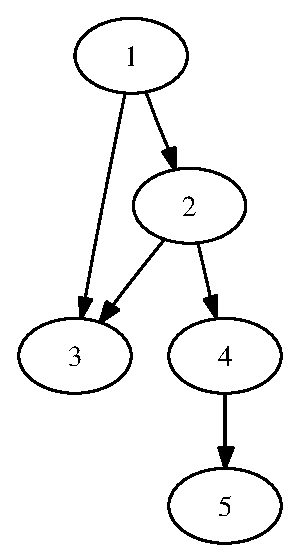
\epsfig{file=Figures/graph0,scale=0.6}

  \caption{Ein einfacher Graph.}
  \label{fig:graph0}
\end{figure}



\noindent
In dem Graphen sind nur die unmittelbaren Verbindungen
zwischen zwei Punkten verzeichnet.  Es gibt aber unter Umst\"{a}nden auch noch
andere Verbindungen.  Beispielsweise gibt es eine unmittelbare Verbindung von
\texttt{1} nach \texttt{3}.  Es gibt dar\"{u}ber hinaus noch einen
Pfad von \texttt{1} nach \texttt{3}, der \"{u}ber den Punkt \texttt{2} geht.  
Unser Ziel in diesem Abschnitt ist es einen Algorithmus zu entwickeln, der \"{u}berpr\"{u}ft, ob
zwischen zwei Punkten eine Verbindung existiert und gegebenenfalls berechnet.
Dazu entwickeln wir zun\"{a}chst einen Algorithmus, der nur \"{u}berpr\"{u}ft, ob es eine
Verbindung zwischen zwei Punkten gibt und erweitern diesen Algorithmus dann sp\"{a}ter so, dass diese
Verbindung auch berechnet wird.

\subsection{Berechnung des transitiven Abschlusses einer Relation}
Als erstes bemerken wir, dass ein Graph $R$ nichts anderes ist als eine bin\"{a}re Relation.
Um feststellen zu k\"{o}nnen, ob es zwischen zwei Punkten eine Verbindung gibt,
m\"{u}ssen wir den transitiven Abschluss $R^+$ der Relation $R$ bilden.  Wir haben bereits
in der Mathematik-Vorlesung gezeigt, dass $R^+$ wie folgt
berechnet werden kann: \\[0.2cm]
\hspace*{1.3cm} $R^+ = \bigcup\limits_{i=1}^{\infty} R^i = R^1 \cup R^2 \cup R^3 \cup \cdots$  \\[0.2cm]
Auf den ersten Blick betrachtet sieht diese Formel so aus, als ob wir unendlich
lange rechnen m\"{u}ssten.  Aber versuchen wir einmal, diese Formel anschaulich zu
verstehen.  Zun\"{a}chst steht da $R$.  Das sind die Verbindungen, die unmittelbar  gegeben
sind.  Als n\"{a}chstes steht dort $R^2$ und das ist $R \circ R$.  Es gilt aber \\[0.2cm]
\hspace*{1.3cm} $R \circ R = \{ \pair(x,z) \mid \exists y \colon \pair(x,y) \in R \wedge \pair(y,z) \in R \}$
\\[0.2cm]
In $R^2$ sind also alle die Pfade enthalten, die aus zwei direkten Verbindungen
zusammengesetzt sind.  Allgemein l\"{a}sst sich durch Induktion sehen, dass $R^n$
alle die Pfade enth\"{a}lt, die aus $n$ direkten Verbindungen zusammengesetzt sind.  Nun
ist die Zahl der Punkte, die wir haben, endlich.  Sagen wir mal, dass es
$k$ Punkte sind.  Dann macht es  keinen Sinn solche Pfade zu betrachten, die
aus mehr als $k-1$ direkten Verbindungen zusammengesetzt sind, denn wir wollen ja
nicht im Kreis herum laufen.  Damit kann dann aber die Formel zur Berechnung des
transitiven Abschlusses vereinfacht werden:\\[0.2cm]
\hspace*{1.3cm} 
$R^+ = \bigcup\limits_{i=1}^{k-1} R^i$.
\\[0.2cm]
Diese Formel k\"{o}nnten wir tats\"{a}chlich so benutzen.  Es ist aber noch effizienter,
einen Fixpunkt-Algorithmus zu verwenden.  Dazu zeigen wir zun\"{a}chst, dass der transitive
Abschluss $R^+$ die folgende Fixpunkt-Gleichung erf\"{u}llt:
\begin{equation}
  \label{fixpunkt}
  R^+ = R \cup R \circ R^+. 
\end{equation}
Wir erinnern hier daran, dass wir vereinbart haben, dass der Operator $\circ$ st\"{a}rker
bindet als der Operator $\cup$, so dass der Ausdruck $R \cup R \circ R^+$ als
$R \cup (R \circ R^+)$ zu lesen ist.
Die Fixpunkt-Gleichung \ref{fixpunkt} l\"{a}sst sich algebraisch beweisen.  Es gilt
\[
\begin{array}{cll}
    & R \cup R \circ R^+ \\[0.2cm]
  = & R \cup R \circ \bigcup\limits_{i=1}^{\infty} R^i \\[0.4cm]
  = & R \cup R \circ \bigl(R^1 \cup R^2 \cup R^3 \cup \cdots \bigr) \\[0.2cm]
  = & R \cup \bigl(R \circ R^1 \cup R \circ R^2 \cup R \circ R^3 \cup \cdots \bigr) &
      \mbox{Distributiv-Gesetz} \\[0.2cm]
  = & R \cup \bigl(R^2 \cup R^3 \cup  R^4 \cup \cdots \bigr) & \mbox{Potenz-Gesetz} \\[0.2cm]
  = & R^1 \cup \bigl(R^2 \cup R^3 \cup  R^4 \cup \cdots \bigr) \\[0.2cm]
  = & \bigcup\limits_{i=1}^{\infty} R^i \\[0.4cm]
  = & R^+
\end{array}
\]
Die Gleichung \ref{fixpunkt} kann benutzt werden um den transitiven Abschluss iterativ zu
berechnen.  Wir definieren eine Folge $(T_n)_{n \in \mathbb{N}}$ durch Induktion folgt:
\begin{enumerate}
\item[I.A.] $n = 1$:         \hspace*{2.3cm} $T_1 := R$
\item[I.S.] $n \mapsto n+1$: \hspace*{1.6cm} $T_{n+1} := R \cup R \circ T_n$. 
\end{enumerate}
Die Relationen $T_n$ lassen sich auf die Relation $R$ zur\"{u}ckf\"{u}hren:
\begin{enumerate}
\item $T_1 = R$.
\item $T_2 = R \cup R \circ T_1 = R \cup R \circ R = R^1 \cup R^2$.
\item $\begin{array}[t]{lcl}
       T_3  & = & R \cup R \circ T_2 \\
            & = & R \cup R \circ (R^1 \cup R^2) \\
            & = & R^1 \cup R^2 \cup R^3. \\
       \end{array}
      $
\end{enumerate}
Allgemein k\"{o}nnen wir durch vollst\"{a}ndige Induktion \"{u}ber $n \in \mathbb{N}$ beweisen, dass
\[ T_n = \bigcup\limits_{i=1}^{n} R^i \]
gilt.  Der Induktions-Anfang folgt unmittelbar aus der Definition von $T_1$.  Um den 
Induktions-Schritt durchzuf\"{u}hren, betrachten wir
\[ \begin{array}{lcll}
   T_{n+1} & = & R \cup R \circ T_n & \mbox{gilt nach Definition} \\[0.2cm]
           & = & R \cup R \circ \left(\bigcup\limits_{i=1}^{n} R^i\right) &
                 \mbox{gilt nach Induktions-Voraussetzung} \\[0.4cm]
           & = & R \cup R^2 \cup \cdots \cup R^{n+1}  &
                 \mbox{Distributiv-Gesetz} \\[0.2cm]
           & = & R^1 \cup \cdots \cup R^{n+1} \\
           & = & \bigcup\limits_{i=1}^{n+1} R^i & \Box 
   \end{array}
\]
Die Folge $(T_n)_{n\in\mathbb{N}}$ hat eine weitere n\"{u}tzliche Eigenschaft: Sie ist 
\emph{monoton steigend}.  Allgemein nennen wir eine Folge von Mengen $(X_n)_{n\in\mathbb{N}}$
\emph{monoton steigend}, wenn 
\\[0.2cm]
\hspace*{1.3cm}
$\forall n \in \mathbb{N}: X_n \subseteq X_{n+1}$
\\[0.2cm]
gilt, wenn also die Mengen $X_n$ mit wachsendem Index $n$ immer gr\"{o}\3er werden.
Die Monotonie der Folge $(T_n)_{n \in \mathbb{N}}$ folgt aus der gerade bewiesenen Eigenschaft
$T_n = \bigcup_{i=1}^{n} R^i$, denn es gilt
\\[0.2cm]
\hspace*{1.3cm}
$
\begin{array}[t]{llcl}
                & T_n \subseteq T_{n+1} \\[0.2cm]
\Leftrightarrow & \bigcup\limits_{i=1}^{n} R^i \subseteq \bigcup\limits_{i=1}^{n+1} R^i \\[0.5cm]
\Leftrightarrow & \bigcup\limits_{i=1}^{n} R^i \subseteq \bigcup\limits_{i=1}^{n} R^i \cup R^{n+1} \\
\end{array}
$
\\[0.2cm]
und die letzte Formel ist offenbar wahr.  Ist nun die Relation $R$ endlich, so ist nat\"{u}rlich 
auch $R^+$ eine endliche Menge.  Da die 
Folge $T_n$ aber in dieser Menge liegt, denn es gilt ja 
\\[0.2cm]
\hspace*{1.3cm}
$T_n = \bigcup\limits_{i=1}^{n} R^i \subseteq \bigcup\limits_{i=1}^{\infty} R^i = R^+$ \quad f\"{u}r alle $n \in \mathbb{N}$,
\\[0.2cm]
k\"{o}nnen die Mengen $T_n$ nicht beliebig gro\3 werden.  Aufgrund der Monotonie der Folge
$(T_n)_{n\in\mathbb{N}}$ muss es daher einen Index $k$ geben, ab dem die Mengen $T_n$ alle gleich sind:
\\[0.2cm]
\hspace*{1.3cm}
$\forall n \in \mathbb{N}:( n \geq k \rightarrow T_n = T_k)$.
\\[0.2cm]
Ber\"{u}cksichtigen wir die Gleichung $T_n = \bigcup_{i=1}^{n} R^i$, so haben wir 
\\[0.2cm]
\hspace*{1.3cm}
$T_n = \bigcup\limits_{i=1}^{n} R^i = \bigcup\limits_{i=1}^{k} R^i = T_k$ \quad f\"{u}r alle $n \geq k$.
\\[0.2cm]
Daraus folgt dann aber, dass
\\[0.2cm]
\hspace*{1.3cm}
$T_n = \bigcup\limits_{i=1}^{n} R^i = \bigcup\limits_{i=1}^{\infty} R^i = R^+$ 
\quad f\"{u}r alle $n \geq k$  
\\[0.2cm]
gilt.  Der Algorithmus zur Berechnung von $R^+$ sieht nun so aus, dass wir die Iteration
\[ T_{n+1} := R \cup R \circ T_n \]
solange durchf\"{u}hren bis $T_{n+1} = T_n$ gilt, denn dann gilt auch $T_n = R^+$.


\begin{figure}[!ht]
  \centering
\begin{Verbatim}[ frame         = lines, 
                  framesep      = 0.3cm, 
                  labelposition = bottomline,
                  numbers       = left,
                  numbersep     = -0.2cm,
                  xleftmargin   = 0.8cm,
                  xrightmargin  = 0.8cm,
                ]
    transClosure := procedure(r) {
        t := r;
        while (true) {
            oldT := t;
            t    := r + product(r, t);
            if (t == oldT) {
                return t;
            }
        }
    };
    product := procedure(r1, r2) {
        return { [x,z] : [x,y] in r1, [y,z] in r2 };
    };
    r := { [1,2], [2,3], [1,3], [2,4], [4,5] };
    print( "r = ", r );
    print( "computing transitive closure of r" );
    t := transClosure(r);
    print( "r+ = ", t );
\end{Verbatim} 
\vspace*{-0.3cm}
\caption{Berechnung des transitiven Abschlusses.}  
\label{fig:transitive-closure.stlx}
\end{figure} %\$

\noindent
Das Programm 
\href{https://github.com/karlstroetmann/Logik/blob/master/SetlX/transitive-closure.stlx}{\texttt{transitive-closure.stlx}}
in Abbildung
\ref{fig:transitive-closure.stlx} auf Seite \pageref{fig:transitive-closure.stlx}  zeigt
eine Implementierung dieses Gedankens.
Lassen wir dieses Programm laufen, so erhalten wir als Ausgabe:
\begin{verbatim}
    R = {[2, 3], [4, 5], [1, 3], [2, 4], [1, 2]}
    R+ = {[1, 5], [2, 3], [4, 5], [1, 4], [1, 3], [2, 4], [1, 2], [2, 5]}
\end{verbatim}
Der transitive Abschluss $R^+$ der Relation $R$ l\"{a}sst sich jetzt anschaulich
interpretieren:  Er enth\"{a}lt alle Paare $\pair(x,y)$, f\"{u}r die es einen \emph{Pfad} von
$x$ nach $y$ gibt.  Ein Pfad von $x$ nach $y$ ist dabei eine Liste der
Form \\[0.2cm]
\hspace*{1.3cm} $\bigl[ x_1, x_2, \cdots, x_n \bigr]$,
\\[0.2cm]
f\"{u}r die $x = x_1$ und $y = x_n$ gilt und f\"{u}r die au\3erdem 
\\[0.2cm]
\hspace*{1.3cm}
$\pair(x_i, x_{i+1}) \in R$ \quad f\"{u}r alle $i = 1, \cdots, n-1$ gilt.
\\[0.2cm]
Die Funktion $\textsl{product}(r_1, r_2)$ berechnet das relationale Produkt $r_1 \circ
r_2$ nach der Formel
\\[0.2cm]
\hspace*{1.3cm}
$r_1 \circ r_2 = \{ \langle x, z \rangle \mid \exists y: \pair(x,y) \in r_1 \wedge \pair(y,z) \in r_2 \}$.
\\[0.2cm]
Die Implementierung dieser Prozedur  zeigt die allgemeine
Form der Mengen-Defi\-nition durch Iteratoren in \textsc{SetlX}.  Allgemein k\"{o}nnen wir eine Menge
durch den Ausdruck
\\[0.2cm]
\hspace*{1.3cm}
$\{\; \textsl{expr} \;\texttt{:}\; [x^{(1)}_1, \cdots, x^{(1)}_{n(1)}] \;\texttt{in}\; s_1,
     \cdots, [x^{(k)}_1, \cdots, x^{(k)}_{n(k)}] \;\texttt{in}\; s_k \;\texttt{|}\;
     \textsl{cond} \;\}
$
\\[0.2cm]
definieren.  Dabei muss $s_i$ f\"{u}r alle $i=1, \cdots, k$ eine Menge von Listen  der L\"{a}nge
$n(i)$ sein.  Bei der Auswertung dieses Ausdrucks werden f\"{u}r die Variablen 
$x^{(i)}_1, \cdots, x^{(i)}_{n(i)}$ die Werte eingesetzt, die die entsprechenden
Komponenten der Listen haben, die in der Menge $s_i$ auftreten.  Beispielsweise w\"{u}rde die
Auswertung von 
\begin{verbatim}
    s1 := { [ 1, 2, 3 ], [ 5, 6, 7 ] };
    s2 := { [ "a", "b" ], [ "c", "d" ] };
    m := { [ x1, x2, x3, y1, y2 ] : [ x1, x2, x3 ] in s1, [ y1, y2 ] in s2 };
\end{verbatim}
f\"{u}r \texttt{m} die Menge
\begin{verbatim}
    { [1, 2, 3, "a", "b"], [5, 6, 7, "c", "d"],  
      [1, 2, 3, "c", "d"], [5, 6, 7, "a", "b"] }
\end{verbatim}
berechnen. 


\subsection{Berechnung der Pfade}
Als n\"{a}chstes wollen wir das Programm zur Berechnung des transitiven Abschlusses so
erweitern, dass wir nicht nur feststellen k\"{o}nnen, dass es einen Pfad zwischen zwei Punkten
gibt, sondern dass wir diesen auch berechnen k\"{o}nnen.  Die Idee ist, dass wir statt des
relationalen Produkts, das f\"{u}r zwei Relationen definiert ist, ein sogenanntes
\emph{Pfad-Produkt}, das auf Mengen von Pfaden definiert ist, berechnen.  Vorab f\"{u}hren wir
f\"{u}r Pfade, die wir ja durch Listen repr\"{a}sentieren,
drei Begriffe ein.
\begin{enumerate}
\item Die Funktion $\textsl{first}(p)$ liefert den ersten Punkt der Liste $p$: \\[0.2cm]
      \hspace*{1.3cm} $\textsl{first}\bigl([x_1,\cdots,x_m]\bigr) = x_1$.
\item Die Funktion $\textsl{last}(p)$ liefert den letzten Punkt der Liste $p$: \\[0.2cm]
      \hspace*{1.3cm} $\textsl{last}\bigl([x_1,\cdots,x_m]\bigl) = x_m$.
\item Sind $p = [ x_1, \cdots, x_m ]$ und $q =[ y_1, \cdots, y_n ]$ 
      zwei Pfade mit $\textsl{first}(q) = \textsl{last}(p)$, dann definieren wir 
      die Summe von $p$ und $q$       als \\[0.2cm]
      \hspace*{1.3cm}
      $p \oplus q := [x_1, \cdots, x_m, y_2, \cdots, y_n ]$.
\end{enumerate}
Sind nun $P_1$ und $P_2$ Mengen von Pfaden, so definieren wir das  \emph{Pfad-Produkt} von
$P_1$ und $P_2$ als \\[0.2cm]
\hspace*{1.3cm} 
$P_1 \bullet P_2 := \bigl\{\; p_1 \oplus p_2 \mid p_1 \in P_1 \wedge p_2 \in P_2 \wedge \textsl{last}(p_1) = \textsl{first}(p_2) \;\bigr\}$.

\begin{figure}[!ht]
  \centering
\begin{Verbatim}[ frame         = lines, 
                  framesep      = 0.3cm, 
                  labelposition = bottomline,
                  numbers       = left,
                  numbersep     = -0.2cm,
                  xleftmargin   = 0.8cm,
                  xrightmargin  = 0.8cm,
                ]
    transClosure := procedure(r) {
        p := r;
        while (true) {
            oldP := p;
            p    := r + pathProduct(r, p);
            if (p == oldP) {
                return p;
            }
        }
    };
    pathProduct := procedure(p, q) {
        return { add(x, y) : x in p, y in q | x[-1] == y[1] };
    };    
    add := procedure(p, q) {
        return p + q[2..];
    };    
    r := { [1,2], [2,3], [1,3], [2,4], [4,5] };
    print( "r = ", r );
    print( "computing all paths" );
    p := transClosure(r);
    print( "p = ", p );
\end{Verbatim} 
\vspace*{-0.3cm}
\caption{Berechnung aller Verbindungen.}  \label{path.stlx}
\end{figure} %\$

\begin{figure}[!ht]
  \centering
  \vspace*{-9cm}

  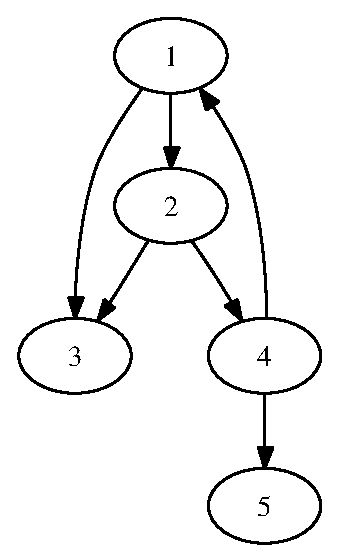
\epsfig{file=Figures/graph-zykl,scale=0.5}
  \vspace*{-1cm}

  \caption{Ein zyklischer Graph.}
  \label{fig:graph-zykl}
\end{figure}

Damit k\"{o}nnen wir das Programm in Abbildung
\ref{fig:transitive-closure.stlx} so ab\"{a}ndern, dass alle m\"{o}glichen Verbindungen zwischen zwei
Punkten berechnet werden.  Abbildung
\ref{path.stlx} zeigt das resultierende Programm
\href{https://github.com/karlstroetmann/Logik/blob/master/SetlX/path.stlx}{\texttt{path.stlx}}. 
Leider funktioniert das Programm dann nicht mehr, wenn der Graph Zyklen enth\"{a}lt.
Abbildung
\ref{fig:graph-zykl} zeigt einen Graphen, der einen Zyklus enth\"{a}lt.  In diesem Graphen
gibt es unendlich viele Pfade, die von dem Punkt 1 zu dem Punkt 2 f\"{u}hren: \\[0.2cm]
\hspace*{1.3cm} $[ 1, 2 ]$, $[ 1, 2, 4, 1, 2 ]$, 
$[ 1, 2, 4, 1, 2, 4, 1, 2 ]$, 
$[ 1, 2, 4, 1, 2, 4, 1, 2, 4, 1, 4 ]$, $\cdots$
\\[0.2cm]
Offenbar  sind die Pfade unwichtig, die einen Punkt mehrfach enthalten und die daher
zyklisch sind.  Solche Pfade sollten wir bei der Berechnung des Pfad-Produktes
eliminieren.

\begin{figure}[!ht]
  \centering
\begin{Verbatim}[ numbers       = left,
                  numbersep     = -0.2cm,
                  frame         = lines, 
                  framesep      = 0.3cm, 
                  labelposition = bottomline,
                  xleftmargin   = 0.0cm,
                  xrightmargin  = 0.0cm,
                ]
    pathProduct := procedure(p, q) {
        return { add(x,y) : x in p, y in q | x[-1] == y[1] && noCycle(x,y) };
    };
    noCycle := procedure(l1, l2) {
        return #({ x : x in l1 } * { x : x in l2 }) == 1;
    };
\end{Verbatim} 
\vspace*{-0.3cm}
\caption{Berechnung aller Verbindungen in zyklischen Graphen}  
\label{fig:path-cyclic.stlx}
\end{figure} %\$

Abbildung \ref{fig:path-cyclic.stlx} zeigt einen Ausschnitt des ge\"{a}nderten Programms
\href{https://github.com/karlstroetmann/Logik/blob/master/SetlX/path-cyclic.stlx}{\texttt{path-cyclic.stlx}},
das auch f\"{u}r zyklische Graphen funktioniert. 
\begin{enumerate}
\item In Zeile 2 ber\"{u}cksichtigen wir nur die Pfade $x \oplus y$, die nicht zyklisch sind.
\item In Zeile 5 \"{u}berpr\"{u}fen wir, ob die Konkatenation  $l_1 \oplus l_2$ zyklisch ist.  Die
      Kombination von $l_1$ und $l_2$  ist genau dann 
      zyklisch, wenn die Listen $l_1$ und $l_2$ mehr als ein gemeinsames Element
      enthalten.  Die Listen $l_1$ und $l_2$ enthalten mindestens ein gemeinsames Element,
      denn wir verkn\"{u}pfen diese beiden Listen ja nur dann, wenn das letzte Element
      der Liste $l_1$ mit dem ersten Element der Liste $l_2$ \"{u}bereinstimmt.
      Wenn es nun noch einen weiteren Punkt geben w\"{u}rde, der sowohl in $l_1$ als auch in
      $l_2$ auftreten w\"{u}rde, dann w\"{a}re der Pfad $l_1 \oplus l_2$ zyklisch.
\end{enumerate}

In den meisten F\"{a}llen sind wird gar nicht daran interessiert, alle m\"{o}glichen Verbindungen
zwischen allen Punkten zu berechnen, das w\"{a}re n\"{a}mlich viel zu aufwendig, sondern wir
wollen nur zwischen zwei gegebenen Punkten 
eine Verbindung finden.  Abbildung \ref{fig:find-path} zeigt die Implementierung einer
Prozedur $\texttt{findPath}(x, y, r)$, die \"{u}berpr\"{u}ft, ob es in dem Graphen $r$ eine
Verbindung von $x$ nach $y$ gibt und die diese Verbindung berechnet.  Das vollst\"{a}ndige
Programm finden Sie in der Datei
\href{https://github.com/karlstroetmann/Logik/blob/master/SetlX/find-path.stlx}{\texttt{find-path.stlx}}.
Wir diskutieren nun die Implementierung der Prozedur \texttt{findPath}.
\begin{enumerate}
\item In Zeile 2 initialisieren wir $p$ so, dass zun\"{a}chst nur der Pfad der L\"{a}nge 0,
      der mit dem Punkt $x$  startet, in $p$ liegt.
\item In Zeile 5 versuchen wir, die Pfade, die wir bereits berechnet haben, mit Hilfe der Relation
      $r$ zu verl\"{a}ngern.  Dabei erhalten wir gegebenenfalls neue Pfade.
\item In Zeile 6 selektieren wir aus allen diesen Pfaden die Pfade aus, die zum Ziel $y$ f\"{u}hren.
\item Wenn wir dann in Zeile 7 feststellen, dass wir einen solchen Pfad berechnet haben,
      geben wir einen dieser Pfade in Zeile 8 zur\"{u}ck.
\item Falls es nicht gelingt einen solchen Pfad zu berechnen und wir keine neuen
      Pfade mehr finden k\"{o}nnen, verlassen wir die Prozedur in Zeile 11
      mit dem Befehl \texttt{return}.  Da wir bei diesem \texttt{return}-Befehl
      keinen Wert zur\"{u}ckgeben, ist der R\"{u}ckgabewert der Prozedur in diesem Fall
      automatisch $\Omega$.
\end{enumerate}

\begin{figure}[!ht]
  \centering
\begin{Verbatim}[ frame         = lines, 
                  framesep      = 0.3cm, 
                  labelposition = bottomline,
                  numbers       = left,
                  numbersep     = -0.2cm,
                  xleftmargin   = 0.8cm,
                  xrightmargin  = 0.8cm,
                ]
    findPath := procedure(x, y, r) {
        p := { [x] };
        while (true) {
            oldP  := p;
            p     := p + pathProduct(p, r);
            found := { l : l in p | l[-1] == y };
            if (found != {}) {
                return arb(found);
            }
            if (p == oldP) {
                return;
            }
        }
    };
\end{Verbatim} 
\vspace*{-0.3cm}
\caption{Berechnung aller Verbindungen zwischen zwei Punkten}  
\label{fig:find-path}
\end{figure}

\subsection{The Wolf, the Goat, and the Cabbage}
Next, we present an application of the theory developed so far.  We show how to solve a problem from
agricultural economy.  The puzzle we want to solve is known as the 
\href{http://jeux.lulu.pagesperso-orange.fr/html/anglais/loupChe/loupChe1.htm}{wolf-goat-cabbage puzzle}:  
\vspace*{0.3cm}

\begin{minipage}[c]{14cm}
{\sl
An agricultural economist has to sell a wolf, a goat, and a cabbage on a market place.  In order to
reach the market place, he has to cross a river.  The boat that he can use is so small that it can
only accommodate either the goat, the wolf, or the cabbage in addition to the agricultural economist.
Now if the agricultural economist leaves the wolf alone with the goat, the wolf will eat the goat.
If, instead, the farmer leaves the goat alone with the cabbage, the goat will eat the cabbage.
Is it possible for the agricultural economist to develop a schedule that allows him to cross the river
without either the goat or the cabbage being eaten?
}
\end{minipage}
\vspace*{0.3cm}

\noindent
In order to compute a schedule, we first have to model the problem.  The various states of the problem will
be regarded as nodes in a graph and this graph will be represented as a binary relation.
To this end we define the set
\\[0.2cm]
\hspace*{1.3cm} 
$\texttt{all} := \{ \squote{farmer}, \squote{wolf}, \squote{goat},\squote{cabbage} \}$.
\\[0.2cm]
Every node will be represented as a subset \texttt{s} of the set \texttt{all}.  The idea is that \texttt{s}
specifies those objects that are on the left side of the river.  We assume that initially the farmer
is on the left side of the river. 
Therefore, the set of all possible states can be defined as the set
\begin{verbatim}
        p := { s : s in 2 ** all | !problem(s) && !problem(all - s) };
\end{verbatim}
Here, we have used the procedure \texttt{problem} to check whether a given set \texttt{s} has a problem. 
Note that since \texttt{s} is the set of objects on the left side, the expression $\texttt{all - s}$
computes the set of objects on the right side of the river.

Next, a set \texttt{s} of objects has a problem if the following conditions
are satisfied:
\begin{enumerate}
\item The farmer is not an element of \texttt{s} and
\item either \texttt{s} contains both the goat and the cabbage or \texttt{s} contains both the wolf and the goat.
\end{enumerate}
Therefore, we can implement the function \texttt{problem} as follows:
\begin{verbatim}
        problem := procedure(s) {
            return !("farmer" in s) &&
                   ("goat" in s && "cabbage" in s || "wolf" in s && "goat" in s);
        };
\end{verbatim}
We proceed to compute the relation \texttt{r} that contains all possible transitions between
different states.  We will compute \texttt{r} using the formula:
\\[0.2cm]
\hspace*{1.3cm}
\texttt{r := r1 + r2;}
\\[0.2cm]
Here \texttt{r1} describes the transitions that result from the farmer crossing the river from left
to right, while \texttt{r2} descibes the transitions that result from the farmer crossing the river
from right to left.  We can define the relation \texttt{r1} as follows:
\begin{verbatim}
        r1  := { [s, s - b]: s in p, b in 2 ** s
                           | s - b in p && "farmer" in b && #b <= 2
               };
\end{verbatim}
Let us explain this definition in detail:
\begin{enumerate}
\item Initially, \texttt{s} is the set of objects on the left side of the river.  Hence, \texttt{s}
      is an element of the set of all states that we have defined as \texttt{p}.
\item \texttt{b} is the set of objects that are put into the boat and that do cross the river.  Of
      course, for an object to go into the boat is has to be on the left side of the river to begin
      with.  Therefore, \texttt{b} is a subset of \texttt{s} and hence an element of the power set
      of \texttt{s}. 
\item Then  \texttt{s-b} is the set of objects that are left on the left side of the river after
      the boat has crossed.  Of course, the new state \texttt{s-b} has to be a state that does not
      have a problem.  Therefore, we check that \texttt{s-b} is an element of \texttt{p}.
\item Furthermore, the farmer has to be in the boat.  This explains the condition 
      \\[0.2cm]
      \hspace*{1.3cm}
      \texttt{\symbol{34}farmer\symbol{34} in b}.
\item Finally, the boat can only have two passengers.  Therefore, we have added the condition
      \\[0.2cm]
      \hspace*{1.3cm}
      \texttt{\#b <= 2}.
\end{enumerate}
Next, we have to define the relation \texttt{r2}.  However, as crossing the river from right to left
is just the reverse of crossing the river from left to right, \texttt{r2} is just the inverse of
\texttt{r1}.   Hence we define:
\\[0.2cm]
\hspace*{1.3cm}
\texttt{r2  := \{ [y, x] : [x, y] in r1 \};}
\\[0.2cm]
Finally, the start state has all objects on the left side.  Therefore, we have
\\[0.2cm]
\hspace*{1.3cm}
\texttt{start := all;}
\\[0.2cm]
In the end, all objects have to be on the right side of the river.  That means that nothing is left
on the left side.  Therefore, we define
\\[0.2cm]
\hspace*{1.3cm}
\texttt{goal := \{\};}
\\[0.2cm]
Figure \ref{fig:wolf-ziege} on page \pageref{fig:wolf-ziege} shows the program
\href{https://github.com/karlstroetmann/Logik/blob/master/SetlX/wolf-goat-cabbage.stlx}{\texttt{wolf-goat-cabbage.stlx}}
that combines the statements shown so far.  The solution computed by this program is shown in Figure
 \ref{fig:wolf-ziege-solution}.

\begin{figure}[!ht]
  \centering
\begin{Verbatim}[ codes         = {\catcode`$=3\catcode`_=8\catcode`^=7},
                  frame         = lines, 
                  framesep      = 0.3cm, 
                  labelposition = bottomline,
                  numbers       = left,
                  numbersep     = -0.2cm,
                  xleftmargin   = 0.8cm,
                  xrightmargin  = 0.8cm,
                ]
    problem := procedure(s) {
        return !("farmer" in s) &&
               ("goat" in s && "cabbage" in s || "wolf" in s && "goat" in s);
    };
   
    all := { "farmer", "wolf", "goat", "cabbage" };
    p   := { s : s in 2 ** all | !problem(s) && !problem(all - s) };
    r1  := { [s, s - b]: s in p, b in 2 ** s
                       | s - b in p && "farmer" in b && #b <= 2
           };
    r2  := { [y, x] : [x, y] in r1 };
    r   := r1 + r2;
    
    start := all;
    goal  := {};
    
    path  := findPath(start, goal, r);
\end{Verbatim} 
\vspace*{-0.3cm}
\caption{Solving the wolf-goat-cabbage problem.}  
\label{fig:wolf-ziege}
\end{figure}


\begin{figure}[!ht]
  \centering
\begin{Verbatim}[ codes         = {\catcode`$=3\catcode`_=8\catcode`^=7},
                  frame         = lines, 
                  framesep      = 0.3cm, 
                  labelposition = bottomline,
                  numbers       = left,
                  numbersep     = -0.2cm,
                  xleftmargin   = 0.8cm,
                  xrightmargin  = 0.8cm,
                ]
    {"cabbage", "farmer", "goat", "wolf"}                                 {}
                             >>>> {"farmer", "goat"} >>>> 
    {"cabbage", "wolf"}                                   {"farmer", "goat"}
                             <<<< {"farmer"} <<<< 
    {"cabbage", "farmer", "wolf"}                                   {"goat"}
                             >>>> {"farmer", "wolf"} >>>> 
    {"cabbage"}                                   {"farmer", "goat", "wolf"}
                             <<<< {"farmer", "goat"} <<<< 
    {"cabbage", "farmer", "goat"}                                   {"wolf"}
                             >>>> {"cabbage", "farmer"} >>>> 
    {"goat"}                                   {"cabbage", "farmer", "wolf"}
                             <<<< {"farmer"} <<<< 
    {"farmer", "goat"}                                   {"cabbage", "wolf"}
                             >>>> {"farmer", "goat"} >>>> 
    {}                                 {"cabbage", "farmer", "goat", "wolf"}
\end{Verbatim} 
\vspace*{-0.3cm}
\caption{A schedule for the agricultural economist.}  
\label{fig:wolf-ziege-solution}
\end{figure}


\section{Terme und Matching}
Neben den bisher vorgestellten Datenstrukturen gibt es noch eine weitere wichtige
Datenstruktur, die sogenannten \emph{Terme}, die insbesondere n\"{u}tzlich ist, wenn wir
\emph{symbolische Programme} 
schreiben wollen.  Darunter verstehen wir solche Programme, die Formeln manipulieren.
Wollen wir beispielsweise ein Programm schreiben, dass als Eingabe einen String wie
\\[0.2cm]
\hspace*{1.3cm}
``\texttt{x * sin(x)}''
\\[0.2cm]
einliest, diesen String als eine Funktion in der Variablen ``\texttt{x}'' interpretiert
und dann die Ableitung dieser Funktion nach der Variablen ``\texttt{x}'' berechnet, so
sprechen wir von einem \emph{symbolischen Programm}.   Wollen wir einen Ausdruck wie 
``\texttt{x * sin(x)}'' darstellen, so eignen sich \emph{Terme} am besten dazu.
Im n\"{a}chsten Unterabschnitt werden wir zun\"{a}chst \emph{Terme} zusammen mit den in \setl\
vordefinierten Funktionen vorstellen, die zur Verarbeitung von Termen benutzt werden k\"{o}nnen.
Anschlie\3end stellen wir das sogenannte \emph{Matching} vor, mit dessen Hilfe sich Terme
besonders leicht manipulieren lassen.


\subsection{Konstruktion und Manipulation von Termen}
Terme werden mit Hilfe sogenannter \emph{Funktions-Zeichen} gebildet.  Es ist wichtig,
dass Sie Funktions-Zeichen nicht mit Funktionen oder Variablen verwechseln.  In \setl\
beginnen Funktionen-Zeichen im Gegensatz zu einem Variablen-Namen daher mit einem gro\3en
Buchstaben.  Auf den Gro\3buchstaben k\"{o}nnen  dann beliebig viele Buchstaben, Ziffern und
der Unterstrich ``\texttt{\_}'' folgen.
Zus\"{a}tzlich gibt es noch Funktionszeichen, die mit dem Zeichen
``\texttt{\symbol{94}}''
beginnen.  Solche Funktions-Zeichen werden intern von \setl\ verwendet um Operator-Symbole
wie ``\texttt{+}'' oder ``\texttt{*}'' darzustellen.
Die folgenden Strings k\"{o}nnen beispielsweise  als Funktions-Zeichen vewendet werden:
\\[0.2cm]
\hspace*{1.3cm}
\texttt{F}, \quad \texttt{FabcXYZ}, \quad \texttt{\symbol{94}sum}, \quad \texttt{Hugo\_}.
\\[0.2cm]
Damit sind wir nun in der Lage, Terme zu definieren.  Ist $F$ ein Funktions-Zeichen und sind
$t_1$, $t_2$, $\cdots$, beliebige \setl-Werte, so ist der Ausdruck
\\[0.2cm]
\hspace*{1.3cm}
$F(t_1, t_2, \cdots, t_n)$
\\[0.2cm]
ein Term.  Beachten Sie, dass Terme ganz \"{a}hnlich aussehen wie die Aufrufe von Funktionen.
Terme und Aufrufe von Funktionen unterscheiden sich nur dadurch, dass bei einem Term links
vor der ersten \"{o}ffnenden Klammer ein Funktions-Zeichen steht, w\"{a}hrend bei einem
Funktions-Aufruf dort statt dessen eine Variable steht, der eine Funktions-Definition zugewiesen
worden ist.

\examples
\begin{enumerate}
\item \texttt{Adresse(\symbol{34}Roteb\"{u}hlplatz 41\symbol{34}, 70178, \symbol{34}Stuttgart\symbol{34})}

      ist ein Term, der eine Adresse repr\"{a}sentiert.
\item \texttt{Product(Variable(\symbol{34}x\symbol{34}), Sin(Variable(\symbol{34}x\symbol{34})))}

      ist ein Term, der einen arithmetischen Ausdruck repr\"{a}sentiert, den Sie mathematisch
      als $x \cdot \sin(x)$ schreiben w\"{u}rden.  \eox
\end{enumerate}

An dieser Stelle fragen Sie sich vielleicht, wie Terme ausgewertet werden.  Die Antwort ist:
\colorbox{red}{Gar nicht!}  Terme werden nur dazu benutzt, Daten darzustellen.  Terme sind also bereits 
Werte  genauso wie auch Zahlen, Strings, Mengen oder Listen als Werte aufgefasst werden.
Genausowenig wie Sie die Zahl \texttt{42} auswerten m\"{u}ssen, m\"{u}ssen Sie einen Term auswerten.

Nehmen wir einmal an,
dass es in \setl\ keine Listen geben w\"{u}rde.  Dann k\"{o}nnten wir Listen als Terme darstellen.  Zun\"{a}chst
w\"{u}rden wir ein Funktions-Zeichen ben\"{o}tigen, mit dem wir die leere Liste darstellen k\"{o}nnten.  Wir
w\"{a}hlen dazu das Funktions-Zeichen \texttt{Nil}.  Damit haben wir dann also die Entsprechung
\\[0.2cm]
\hspace*{1.3cm}
$\texttt{Nil}() \;\widehat{=}\; \texttt{[]}$.
\\[0.2cm]
\textbf{Beachten} Sie hier, dass die Klammern hinter dem Funktions-Zeichen \texttt{Nil} nicht
weggelassen werden d\"{u}rfen!  Um nun eine Liste darzustellen, deren erstes Element $x$ ist und deren
restliche Elemente durch die Restliste $r$ gegeben sind, verwenden wir das Funktions-Zeichen
\texttt{Cons}.  Dann haben wir die Entsprechung
\\[0.2cm]
\hspace*{1.3cm}
$\texttt{Cons(x, r)} \;\widehat{=}\; \texttt{[}x\texttt{]}+r$. 
\\[0.2cm]
Konkret k\"{o}nnen wir nun die Liste \texttt{[1,2,3]} durch den Term
\\[0.2cm]
\hspace*{1.3cm}
\texttt{Cons(1, Cons(2, Cons(3, Nil())))}
\\[0.2cm]
darstellen.  In der Sprache \textsl{Prolog}, werden Listen intern in \"{a}hnlicher Form als Terme dargestellt.

Es gibt zwei vordefinierte Funktionen in \setl, mit denen wir auf die Komponenten eines Terms
zugreifen k\"{o}nnen und es gibt eine weitere Funktion, mit deren Hilfe wir Terme konstruieren k\"{o}nnen.
\begin{enumerate}
\item Die Funktion \texttt{fct} berechnet das Funktions-Zeichen eines Terms.
      Falls $t$ ein Term der Form $F(s_1,\cdots,s_n)$ ist, so ist das Ergebnis des Funktions-Aufrufs
      \\[0.2cm]
      \hspace*{1.3cm}
      $\texttt{fct}(F(s_1,\cdots,s_n))$
      \\[0.2cm]
      das Funktions-Zeichen $F$ dieses Terms.  Beispielsweise liefert der Ausdruck
      \\[0.2cm]
      \hspace*{1.3cm}
      \texttt{fct(Cons(1, Cons(2, Cons(3, Nil()))))}
      \\[0.2cm]
      als Ergebnis das Funktions-Zeichen \texttt{\symbol{34}Cons\symbol{34}}.
\item Die Funktion \texttt{args} berechnet die Argumente eines Terms.
      Falls $t$ ein Term der Form $F(s_1,\cdots,s_n)$ ist, dann liefert der Ausdruck
      \\[0.2cm]
      \hspace*{1.3cm}
      $\mathtt{args}(F(s_1,\cdots,s_n))$
      \\[0.2cm]
      als Ergebnis die Liste $[s_1, \cdots, s_n]$ der Argumente des Terms $t$  .  Beispielsweise
      liefert der Ausdruck
      \\[0.2cm]
      \hspace*{1.3cm}
      \texttt{args(Cons(1, Cons(2, Cons(3, Nil()))))}
      \\[0.2cm]
      das Ergebnis
      \\[0.2cm]
      \hspace*{1.3cm}
      \texttt{[1, Cons(2, Cons(3, Nil()))]}.
\item Ist ein Funktions-Zeichen $f$ und eine Liste $l$ von Argumenten gegeben, so erzeugt die
      Funktion \texttt{makeTerm} durch den Aufruf
      \\[0.2cm]
      \hspace*{1.3cm}
      $\texttt{makeTerm}(f,l)$
      \\[0.2cm]
      einen Term $t$ mit dem Funktions-Zeichen $f$ und der Argument-Liste $l$, f\"{u}r $t$ gilt also
      \\[0.2cm]
      \hspace*{1.3cm}
      $\mathtt{fct}(t) = f$  \quad und \quad $\mathtt{args}(t) = l$.
      \\[0.2cm]
      Beispielsweise liefert der Aufruf
      \\[0.2cm]
      \hspace*{1.3cm}
      \texttt{makeTerm(\symbol{34}Cons\symbol{34}, [ 1, Nil() ])}
      \\[0.2cm]
      als Ergebnis den Term
      \\[0.2cm]
      \hspace*{1.3cm}
      \texttt{Cons(1,Nil())}.
      \\[0.2cm]
      Diesen Term h\"{a}tten wir nat\"{u}rlich auch unmittelbar hinschreiben k\"{o}nnen.
\end{enumerate}

\begin{figure}[!ht]
\centering
\begin{Verbatim}[ frame         = lines, 
                  framesep      = 0.3cm, 
                  firstnumber   = 1,
                  labelposition = bottomline,
                  numbers       = left,
                  numbersep     = -0.2cm,
                  xleftmargin   = 0.8cm,
                  xrightmargin  = 0.8cm,
                ]
    append := procedure(l, x) {
        if (fct(l) == "Nil") {
            return Cons(x, Nil());
        }
        [head, tail] := args(l);
        return Cons(head, append(tail, x));
    };
\end{Verbatim}
\vspace*{-0.3cm}
\caption{Einf\"{u}gen eines Elements am Ende einer Liste.}
\label{fig:append.stlx}
\end{figure}

In Abbildung  \ref{fig:append.stlx} auf Seite \pageref{fig:append.stlx} sehen Sie die
Implementierung  einer Funktion
\href{https://github.com/karlstroetmann/Logik/blob/master/SetlX/append.stlx}{\texttt{append}},
deren Aufgabe es ist, ein Element $x$ am Ende einer Liste $l$ einzuf\"{u}gen, wobei vorausgesetzt ist,
dass die Liste $l$ als Term mit Hilfe der Funktions-Zeichen ``\texttt{Cons}'' und ``\texttt{Nil}''
dargestellt wird.
\begin{enumerate}
\item Zun\"{a}chst wird in Zeile 2 \"{u}berpr\"{u}ft, ob die Liste $l$ leer ist.  Die Liste $l$ ist genau dann
      leer, wenn $l = \texttt{Nil()}$ gilt.  Daher k\"{o}nnen wir einfach das Funktions-Zeichen des
      Terms $l$ testen um herauszufinden, ob $l$ die leere Liste repr\"{a}sentiert.
\item Falls $l$ nicht leer ist, muss $l$ die Form
      \\[0.2cm]
      \hspace*{1.3cm}
      $l = \texttt{Cons(\textsl{head}, \textsl{tail})}$
      \\[0.2cm]     
      haben.  Dann ist \textsl{head} das erste Element der Liste $l$ und \textsl{tail} bezeichnet
      die Liste der restlichen Elemente.  In diesem Fall m\"{u}ssen wir $x$ rekursiv in die Liste
      \textsl{tail} einf\"{u}gen.  Als Ergebnis wird in Zeile 6 dann eine neue Liste erzeugt, deren
      erstes Element \textsl{head} ist, w\"{a}hrend die Liste der restlichen Elemente durch den
      rekursiven Aufruf von \textsl{append} berechnet wird.
\end{enumerate}
In manchen F\"{a}llen ist es sehr unbequem, dass Funktions-Zeichen immer mit einem gro\3en Buchstaben
beginnen m\"{u}ssen.  Deswegen gibt es in \setl\ einen Escape-Mechanismus, der es erlaubt, auch
Funktionszeichen zu verwenden, die mit einem kleinen Buchstaben beginnen:  Falls wir einem
Funktionszeichen den Operator ``\texttt{\symbol{64}}'' voranstellen, dann darf das Funktionszeichen
auch mit einem kleinen Buchstaben beginnen.  Wollen wir beispielsweise Terme benutzen um
algebraische Ausdr\"{u}cke darzustellen, die trigonometrische Funktionen enthalten, 
so k\"{o}nnen wir einen Ausdruck der Form $\sin(x)$ durch den Term
\\[0.2cm]
\hspace*{1.3cm}
\texttt{\symbol{64}sin(\symbol{34}x\symbol{34})}  
\\[0.2cm]
darstellen.

\subsection{Matching}
Der Umgang mit Termen w\"{a}re sehr m\"{u}hsam, wenn wir die Terme jedesmal mit Hilfe der Funktionen
\texttt{fct} und \texttt{args} auseinander nehmen m\"{u}ssten.  Abbildung \ref{fig:append-match.stlx} 
zeigt eine weitere Implementierung der Funktion
\href{https://github.com/karlstroetmann/Logik/blob/master/SetlX/append-match.stlx}{\texttt{append}}, 
bei der wir die Kontroll-Struktur \texttt{match} an Stelle der Funktionen ``\texttt{fct}''
and ``\texttt{args}'' verwendet haben.  In Zeile 3 wird  \"{u}berpr\"{u}ft, ob die Liste $l$ leer ist.
Die wahre St\"{a}rke des Matchings sehen wir allerdings ist in Zeile 4, denn dort wird nicht nur
\"{u}berpr\"{u}ft, ob die Liste $l$ die Form
\\[0.2cm]
\hspace*{1.3cm}
\texttt{Cons(\textsl{head},\textsl{tail})}
\\[0.2cm]
hat, sondern gleichzeitig werden die Variablen \textsl{head} and \textsl{tail} so gesetzt, dass
anschlie\3end die Gleichung
\\[0.2cm]
\hspace*{1.3cm}
$l = \texttt{Cons(\textsl{head},\textsl{tail})}$
\\[0.2cm]
erf\"{u}llt ist.


\begin{figure}[!ht]
\centering
\begin{Verbatim}[ frame         = lines, 
                  framesep      = 0.3cm, 
                  firstnumber   = 1,
                  labelposition = bottomline,
                  numbers       = left,
                  numbersep     = -0.2cm,
                  xleftmargin   = 0.8cm,
                  xrightmargin  = 0.8cm,
                ]
    append := procedure(l, x) {
        match (l) {
            case Nil():            return Cons(x, Nil());
            case Cons(head, tail): return Cons(head, append(tail, x));
        }
    };
\end{Verbatim}
\vspace*{-0.3cm}
\caption{Implementierung von \texttt{append} mit Hilfe von \emph{Matching}.}
\label{fig:append-match.stlx}
\end{figure}

Im Allgemeinen ist  ein \texttt{match}-Block so \"{a}hnlich aufgebaut wie ein
\texttt{switch}-Block und hat die in Abbildung \ref{fig:match} gezeigte Struktur.
Hier bezeichnet $e$ einen Ausdruck, dessen Auswertung einen Term ergibt.  
Die Ausdr\"{u}cke $t_1$, $\cdots$, $t_n$ sind sogenannte \emph{Muster}, die freie
Variablen enthalten.  Bei der Auswertung eines \texttt{Match}-Blocks versucht
\textsc{SetlX} die in dem Muster $t_i$ auftretenden Variablen so zu setzen, dass das Muster
zu dem Ergebnis der Auswertung von $e$ gleich ist.  Gelingt dies, so wird die
mit $\textsl{body}_i$ bezeichnete Gruppe von Befehlen ausgef\"{u}hrt.  Andernfalls
versucht \textsc{SetlX} das n\"{a}chste Muster $t_{i+1}$ mit $e$ zur Deckung zu bringen.
Falls keines der Muster $t_1$, $\cdots$, $t_n$ mit $e$ zur Deckung zu bringen ist, wird
ersatzweise $\textsl{body}_{n+1}$ ausgef\"{u}hrt.  

\begin{figure}[!ht]
  \centering
\begin{Verbatim}[ codes         = {\catcode`_=8\catcode`^=7},
                  frame         = lines, 
                  framesep      = 0.3cm, 
                  labelposition = bottomline,
                  numbers       = left,
                  numbersep     = -0.2cm,
                  commandchars  = \\\{\},
                  xleftmargin   = 0.8cm,
                  xrightmargin  = 0.8cm
                ]
      \texttt{\underline{match} (\(e\)) \{}
          \texttt{\underline{case}} \(t_1\) : \textsl{body}\(_1\) 
          \vdots
          \texttt{\underline{case}} \(t_n\) : \textsl{body}\(_n\)
          \texttt{\underline{default}:} \textsl{body}\(_{n+1}\)
      \texttt{\}}
\end{Verbatim}
\vspace*{-0.3cm}
\caption{Struktur eines \texttt{Match}-Blocks}  \label{fig:match}
\end{figure} 


\begin{figure}[!ht]
\centering
\begin{Verbatim}[ frame         = lines, 
                  framesep      = 0.3cm, 
                  firstnumber   = 1,
                  labelposition = bottomline,
                  numbers       = left,
                  numbersep     = -0.2cm,
                  xleftmargin   = 0.8cm,
                  xrightmargin  = 0.8cm,
                ]
    diff := procedure(t, x) {
        match (t) {
            case t1 + t2 :
                return diff(t1, x) + diff(t2, x);
            case t1 - t2 :
                return diff(t1, x) - diff(t2, x);
            case t1 * t2 :
                return diff(t1, x) * t2 + t1 * diff(t2, x);
            case t1 / t2 :
                return ( diff(t1, x) * t2 - t1 * diff(t2, x) ) / t2 * t2;
            case f ** g :
                return diff( @exp(g * @ln(f)), x);
            case ln(a) :
                return diff(a, x) / a;
            case exp(a) :
                return diff(a, x) * @exp(a);
            case ^variable(x) : // x is defined above as second argument
                return 1;
            case ^variable(y) : // y not yet defined, matches any other variable
                return 0;
            case n | isNumber(n):   
                return 0;  
        }
    };
\end{Verbatim}
\vspace*{-0.3cm}
\caption{A function to perform symbolic differentiation.}
\label{fig:diff.stlx}
\end{figure}

\noindent
Wir zeigen zum Abschluss dieses Abschnitts ein komplexeres Beispiel.  Die in Abbildung
\ref{fig:diff.stlx} auf Seite \pageref{fig:diff.stlx} gezeigte Funktion
\href{https://github.com/karlstroetmann/Logik/blob/master/SetlX/diff.stlx}{\texttt{diff}}
wird mit zwei Argumenten aufgerufen:
\begin{enumerate}
\item Das erste  Argument $t$ ist ein Term, der einen arithmetischen Ausdruck repr\"{a}sentiert.
\item Das zweite Argument $x$ ist ein String, der als Variable interpretiert wird.
\end{enumerate}
Die Aufgabe der Funktion \texttt{diff} besteht darin, den durch $t$ gegebenen Ausdruck nach der
in $x$ angegebenen Variablen zu differenzieren.  Wollen wir beispielsweise die Funktion
\\[0.2cm]
\hspace*{1.3cm}
$x \mapsto x^x$
\\[0.2cm]
nach $x$ ableiten, so k\"{o}nnen wir die Funktion \texttt{diff} wie folgt aufrufen.
\\[0.2cm]
\hspace*{1.3cm}
\texttt{diff(parse(\symbol{34}x ** x\symbol{34}), \symbol{34}x\symbol{34});}
\\[0.2cm]
Hier wandelt die Funktion \texttt{parse} den String ``\texttt{x ** x}'' in einen Term um.  Die
genaue Struktur dieses Terms diskutieren wir weiter unten.  Wir betrachten
zun\"{a}chst den \texttt{match}-Befehl in  Abbildung \ref{fig:diff.stlx}.  
In Zeile  3 hat der zu differenzierende Ausdruck die Form
\texttt{t1 + t2}.  Um einen solchen Ausdruck nach einer Variablen $x$ zu differenzieren, m\"{u}ssen wir
sowohl  \texttt{t1} als auch \texttt{t2} nach $x$ differenzieren.  Die dabei erhaltenen Ergebnisse
sind dann zu addieren.  Etwas interessanter ist Zeile 8, welche die Produkt-Regel der
Differenzial-Rechnung umsetzt.  Die Produkt-Regel lautet:
\\[0.2cm]
\hspace*{1.3cm}
$\displaystyle \frac{d\;}{dx} \bigl(t_1 \cdot t_2\bigr) = \frac{d\, t_1}{dx} \cdot t_2 + t_1 \cdot \frac{d\,t_2}{dx}$.
\\[0.2cm]
Bemerken Sie, dass in Zeile 7 das Muster
\\[0.2cm]
\hspace*{1.3cm}
\texttt{t1 * t2}
\\[0.2cm]
zum einen dazu dient, zu erkennen, dass der zu differenzierende Ausdruck ein Produkt ist, zum
anderen aber auch die beiden Faktoren des Produkts extrahiert und an die Variablen $t_1$ und $t_2$ bindet.
In den Zeilen  12 und 16 haben wir den Funktions-Zeichen ``\texttt{exp}'' und ``\texttt{ln}'' den
 Operator ``\texttt{\symbol{64}}'' vorangestellen m\"{u}ssen, denn sonst w\"{u}rden die Strings
 ``\texttt{exp}'' und ``\texttt{ln}'' nicht als Funktions-Zeichen sondern als Variablen
 aufgefasst werden. 

Die Regel zur Berechnung der  Ableitung eines Ausdrucks der Form $f^g$ beruht auf der
Gleichung
\\[0.2cm]
\hspace*{1.3cm}
$f^g = \exp\bigl(\ln\bigl(f^g\bigr)\bigr) = \exp\bigl(g \cdot \ln(f)\bigr)$,
\\[0.2cm]
die in Zeile 12 umgesetzt wird.  

Um einen Ausdruck der Form $\ln(f)$ abzuleiten, m\"{u}ssen
wir die Kettenregel anwenden.  Da $\frac{d\;}{dx} \ln(x) = \frac{1}{x}$ ist, haben wir insgesamt
\\[0.2cm]
\hspace*{1.3cm}
$\displaystyle \frac{d\;}{dx} \ln(f) = \frac{1}{f} \cdot \frac{d\,f}{dx}$.
\\[0.2cm]
Diese Gleichung wurde in Zeile 14 verwendet.  In analoger Weise wird dann in Zeile 16 mit Hilfe der
Kettenregel ein Ausdruck der Form $\mathtt{exp}(f)$ abgeleitet.

Um das Beispiel in Abbildung \ref{fig:diff.stlx} besser zu verstehen m\"{u}ssen wir wissen, 
wie die Funktion \texttt{parse} einen String in einen Term umwandelt.  Die Funktion 
 \texttt{parse} muss sowohl Operator-Symbole als auch Variablen verarbeiten.
Eine Variable der Form  \texttt{\symbol{34}x\symbol{34}} wird in den Term
\\[0.2cm]
\hspace*{1.3cm}
\texttt{\symbol{94}variable(\symbol{34}x\symbol{34})}
\\[0.2cm]
umgewandelt.  Dies erkl\"{a}rt die Zeilen 19 und 21 von Abbildung \ref{fig:diff.stlx}.

Wir k\"{o}nnen die interne Darstellung eines Terms mit Hilfe der Funktion
``\texttt{canonical}'' ausgeben.  Beispielsweise liefert der Ausdruck
\\[0.2cm]
\hspace*{1.3cm}
\texttt{canonical(parse(\symbol{34}x ** x\symbol{34}))}
\\[0.2cm]
das Ergebnis
\\[0.2cm]
\hspace*{1.3cm}
\texttt{\symbol{94}power(\symbol{94}variable(\symbol{34}x\symbol{34}), \symbol{94}variable(\symbol{34}x\symbol{34}))}.
\\[0.2cm]
Dies zeigt, dass der Exponentiations-Operator ``\texttt{**}'' in \setl\ intern durch das Funktions-Zeichen
``\texttt{\symbol{94}power}'' dargestellt wird.  Die interne Darstellung des Operators
``\texttt{+}'' ist ``\texttt{\symbol{94}sum}'',
``\texttt{-}'' wird durch das Funktions-Zeichen ``\texttt{\symbol{94}difference}'' dargestellt,
``\texttt{*}'' wird durch das Funktions-Zeichen ``\texttt{\symbol{94}product}'' dargestellt und der Operator
``\texttt{/}'' wird durch das Funktions-Zeichen ``\texttt{\symbol{94}quotient}'' dargestellt.

Terme sind in dem folgenden Sinne \emph{viral}:  Falls ein Argument eines der Operatoren
``\texttt{+}'', ``\texttt{-}'', ``\texttt{*}'', ``\texttt{/}'', ``\texttt{\symbol{92}}'' und
``\texttt{\%}''
ein Term ist, so erzeugt der Operator als Ergebnis automatisch einen Term.
Beispielsweise liefert der Ausdruck
\\[0.2cm]
\hspace*{1.3cm}
\texttt{parse(\symbol{34}x\symbol{34}) + 2}
\\[0.2cm]
den Term
\\[0.2cm]
\hspace*{1.3cm}
\texttt{\symbol{94}sum(\symbol{94}variable(\symbol{34}x\symbol{34}), 2)}.
\\[0.2cm]
Zeile 21 zeigt, dass an ein Muster in einem \texttt{case} eine Bedingung angeschlossen werden kann:
Das Muster
\\[0.2cm]
\hspace*{1.3cm}
\texttt{case n:}
\\[0.2cm]
passt zun\"{a}chst auf jeden Term.  Allerdings wollen wir in Zeile 21 nur Zahlen matchen.  Daher haben
wir an dieses Muster mit Hilfe des Operators ``\texttt{|}'' noch die Bedingung \texttt{isNumber(n)}
angeh\"{a}ngt, mit der wir sicherstellen, dass $n$ tats\"{a}chlich eine Zahl ist.


\subsection{Ausblick}
Wir konnten in diesem einf\"{u}hrenden Kapitel nur einen Teil der Sprache \textsc{SetlX}
behandeln.  Einige weitere Features
der Sprache \textsc{SetlX} werden wir noch in den folgenden Kapiteln diskutieren.
Zus\"{a}tzlich finden Sie
weitere Informationen  in dem Tutorial, das im Netz unter der Adresse
\\[0.2cm]
\hspace*{1.3cm}
\href{https://github.com/karlstroetmann/setlX/blob/master/tutorial.pdf}{\texttt{https://github.com/karlstroetmann/setlX/blob/master/tutorial.pdf}}
\\[0.2cm]
abgelegt ist.  

\remark
Die meisten der in diesem Abschnitt vorgestellten Algorithmen sind 
nicht effizient.  Sie dienen nur dazu, die Begriffsbildungen aus der Mengenlehre konkret
werden zu lassen.  Die Entwicklung effizienter Algorithmen ist Gegenstand des zweiten
Semesters. 


%%% Local Variables: 
%%% mode: latex
%%% TeX-master: "logik"
%%% End: 

